\subsection{\texorpdfstring{格罗滕迪克群 \(R_{K}(A)\)}{格罗滕迪克群 R\_\{K\}(A)}}

设 \(\mathrm{K}\) 是一个交换域，\(\mathrm{A}\) 是一个 \(\mathrm{K}\)-代数。在 \(\mathrm{K}\) 上为有限维向量空间的 A-模的类所成之集是遗传的。相应的格罗滕迪克群记作 \(\mathrm{R}_{\mathrm{K}}(\mathrm{A})\)。它是一个自由 \(\mathbf{Z}\)-模，以族 \(([\mathrm{S}])_{\mathrm{S}\in \mathcal{S}}\) 为基，其中 \(\mathcal{S}\) 是在 \(\mathrm{K}\) 上为有限维的单 A-模的类所成之集。存在一个同态

\[
\dim : \mathrm{R} _ {\mathrm{K}} (\mathrm{A}) \longrightarrow \mathbf {Z}
\]

它由条件 \(\dim([E]) = [E : K]\)（对每个在 K 上为有限维的 A-模 E）刻画。当 A = K 时，它是一个同构。有效元所成的子幺半群记作 \(\mathrm{R}_{\mathrm{K}}(\mathrm{A})^{+}\)。

引理 2. —— 设 M 与 M' 是在 K 上为有限维向量空间的 A-模。M 与 M' 的支集（VIII, 第 190 页）不相交当且仅当存在 \(a \in A\)，使得 \(a_{M} = 0_{M}\) 且 \(a_{M'} = 1_{M'}\)。

假设存在 \(a \in \mathrm{A}\)，使得 \(a_{\mathrm{M}} = 0_{\mathrm{M}}\) 且 \(a_{\mathrm{M}'} = 1_{\mathrm{M}'}\)。设 S 是一个单 A-模。若 \(\operatorname{cl}(S)\) 属于 M 的支集 \(\mathcal{S}_{\mathrm{M}}\)，则 A-模 S 同构于 M 的某条若尔当–赫尔德列的商之一，且我们有 \(a_{\mathrm{S}} = 0_{\mathrm{S}}\)。同样，若 \(\operatorname{cl}(S)\) 属于 \(\mathcal{S}_{\mathrm{M}'}\)（即 \(\mathrm{M}'\) 的支集），则我们有 \(a_{\mathrm{S}} = 1_{\mathrm{S}}\)。由此得出 \(\mathcal{S}_{\mathrm{M}}\) 与 \(\mathcal{S}_{\mathrm{M}'}\) 不相交。

反之，假设集 \(S_{M}\) 与 \(S_{M'}\) 不相交。由于 M 与 \(M'\) 在 K 上是有限维的，它们是有限的。类属于 \(S_{M} \cup S_{M'}\) 的每个单 A-模 S 在 K 上是有限维的，从而更是在体 \(\operatorname{End}_{\mathrm{A}}(\mathrm{S})\) 上有限维。由命题 4 的推论 1（VIII, 第 83 页），存在元素 \(b \in A\)，使得有 \(b_{S} = 0_{S}\)（相应地，\(b_{S} = 1_{S}\)）对每个类属于 \(S_{M}\)（相应地，\(S_{M'}\)）的单 A-模 S 成立。设 \((\mathrm{M}_{i})_{0 \leqslant i \leqslant n}\) 是 M 的一条若尔当–赫尔德列。由前所述，我们有 \(bM_{i} \subset M_{i+1}\)（对 \(0 \leqslant i < n\)），因而 \((b^{n})_{\mathrm{M}} = 0_{\mathrm{M}}\)。使得 \(((1-b)^{m})_{\mathrm{M}^{\prime}}=0_{\mathrm{M}^{\prime}}\) 的自然数 m 的存在性用同样方式证明。令 \(\mathrm{P}(\mathrm{X})=1-(1-\mathrm{X}^{n})^{m}\) 且 \(a=\mathrm{P}(b)\)。多项式 \(\mathrm{P}(\mathrm{X})\) 是 \(X^{n}\) 的倍式，故我们有 \(a_{M}=0_{M}\)，而多项式 \(1-\mathrm{P}(\mathrm{X})\) 是 \((1-\mathrm{X})^{m}\) 的倍式，故我们有 \(a_{M^{\prime}}=1_{M^{\prime}}\)。证明至此完成。

设 \(\mathrm{L}\) 是 \(\mathrm{K}\) 的一个扩张。若 \(\mathrm{M}\) 是一个在 \(\mathrm{K}\) 上为有限维的 A-模，则 \(\mathrm{M}_{(\mathrm{L})}\) 是一个 \(\mathrm{A}_{(\mathrm{L})}\)-模，且在 \(\mathrm{L}\) 上为有限维。此外，对 A-模的每个正合列

\[
0 \longrightarrow \mathrm{M} ^ {\prime} \longrightarrow \mathrm{M} \longrightarrow \mathrm{M} ^ {\prime \prime} \longrightarrow 0
\]

（由 A-模组成），由它经标量扩张导出的 \(A_{(L)}\) -模的序列

\[
0 \longrightarrow \mathrm{M} _ {(\mathrm{L})} ^ {\prime} \longrightarrow \mathrm{M} _ {(\mathrm{L})} \longrightarrow \mathrm{M} _ {(\mathrm{L})} ^ {\prime \prime} \longrightarrow 0
\]

是正合的（II, §7, No.~7, 第 308 页，命题 14）。因此，存在唯一的环同态 \(u: \mathrm{R}_{\mathrm{K}}(\mathrm{A}) \to \mathrm{R}_{\mathrm{L}}(\mathrm{A}_{(\mathrm{L})})\)，使得对每个在 K 上为有限维的 A-模 M，有 \(u([\mathrm{M}]) = [\mathrm{M}_{(\mathrm{L})}]\)（No.~5）。

定理 1. —— 上面定义的同态 \(u: \mathrm{R}_{\mathrm{K}}(\mathrm{A}) \to \mathrm{R}_{\mathrm{L}}(\mathrm{A}_{(\mathrm{L})})\) 是单射。设 \(\xi\) 是 \(\mathrm{R}_{\mathrm{K}}(\mathrm{A})\) 的一个元素。则 \(\xi\) 是有效的当且仅当 \(u(\xi)\) 是有效的。

引理 3. —— 设 S 与 T 是两个在 K 上为有限维的互不同构的单 A-模。\(\mathrm{A}_{(\mathrm{L})}\)-模 \(\mathrm{S}_{(\mathrm{L})}\) 与 \(\mathrm{T}_{(\mathrm{L})}\) 的支集不相交。

由引理 2，存在元素 \(a \in \mathrm{A}\)，使得 \(a_{\mathrm{S}} = 0\) 且 \(a_{\mathrm{T}} = 1\)。元素 \(1 \otimes a\)（它属于 \(\mathrm{A}_{(\mathrm{L})}\)）在 \(\mathrm{S}_{(\mathrm{L})}\) 上作用为 0，在 \(\mathrm{T}_{(\mathrm{L})}\) 上作用为 1。由引理 2，\(\mathrm{A}_{(\mathrm{L})}\)-模 \(\mathrm{S}_{(\mathrm{L})}\) 与 \(\mathrm{T}_{(\mathrm{L})}\) 的支集不相交。

我们来证明定理 1。用 S 表示在 K 上为有限维的单 A-模的类所成之集。族 \(([S])_{S \in \mathcal{S}}\) 是 Z-模 \(R_{K}(A)\) 的一个基。设 \(S \in S\)。\(A_{(L)}\)-模 \(S_{(L)}\) 非零，故其支集非空。设 \(S'\) 是该支集的一个元素。由 VIII, 第 190 页的引理 1，存在同态 \(f_{S'} : R_L(A_{(L)}) \to Z\)，使得 \(f_{S'}([E]) = \ell_{S'}(E)\) 对每个在 L 上为有限维的 \(A_{(L)}\)-模 E 成立。按构造我们有 \(f_{S'}([S_{(L)}]) \neq 0\)，且由引理 3，有 \(f([T_{(L)}]) = 0\) 对每个 \(T \in S - \{S\}\) 成立。于是我们证明了：\(R_L(A_{(L)})\) 中形如 \([S_{(L)}]\)（\(S \in S\)）的元素在 Z 上线性无关。由此推出同态 u 是单射。

设 \(S \in \mathscr{S}\)，且设 \(S'\) 是 \(S_{(L)}\) 的支集的一个元素。对每个 \(\xi \in R_K(A)\)，\(\xi\) 的以下标 {[}S{]} 为指标的坐标（在基 \(([S])_{S \in \mathscr{S}}\) 中）是 \(f_{S'}(u(\xi)) / [S_{(L)} : S']\)。由此得出：若 \(u(\xi)\) 是有效的，则 \(\xi\) 也是有效的。

\subsection{K(C) 上的乘法结构}

设 K 是一个交换环，A 是环 K 上的一个双代数（III, §11, No.~4, 第 585 页），其余积为 c，余单位为 \(\gamma\)。除非另有说明，张量积都是在 K 上取的。设 E 与 F 是（左）A-模。张量积 \(E \otimes F\) 赋有一个 \((A \otimes A)\)-模结构，它由公式

\[
(a \otimes b) (x \otimes y) = a x \otimes b y\tag{11}
\]

（对 \(a, b \in \mathrm{A}\)，\(x \in \mathrm{E}\)，\(y \in \mathrm{F}\)）刻画。利用同态 \(c: \mathrm{A} \to \mathrm{A} \otimes \mathrm{A}\)，我们从这个 \((\mathrm{A} \otimes \mathrm{A})\)-模导出一个 A-模 \(c_*(\mathrm{E} \otimes \mathrm{F})\)（II, §1, No.~13, 第 221 页）。更精确地说，设 \(a \in \mathrm{A}\)；若 \(c(a) = \sum_{i} a_{i} \otimes b_{i}\)，则我们有

\[
a (x \otimes y) = \sum_ {i} a _ {i} x \otimes b _ {i} y\tag{12}
\]

（对 \(x \in E\)，\(y \in F\)）成立。记号滥用起见，我们也把这样得到的 A-模记作 \(E \otimes F\)。由 c 的余结合性立即得出，K-模的典范同构

\[
\varphi : (\mathrm{E} \otimes \mathrm{F}) \otimes \mathrm{G} \longrightarrow \mathrm{E} \otimes (\mathrm{F} \otimes \mathrm{G})
\]

对一切 A-模 E、F、G 都是 A-线性的。同样，若双代数 A 是余交换的，则从 \(E \otimes F\) 到 \(F \otimes E\) 的典范同构是 A-线性的。最后，用 \(K_{\gamma}\) 表示以加群 K 为底群、外部合成律为 \((a, x) \mapsto \gamma(a)x\) 的 A-模。从 \(K \otimes E\)（相应地，\(E \otimes K\)）到 E 的典范同构是从 \(K_{\gamma} \otimes E\)（相应地，\(E \otimes K_{\gamma}\)）到 E 的 A-模同构。

命题 9. —— 设 K 是一个交换环，A 是 K 上余单位为 γ 的一个双代数，C 是 A-模的类的一个加性集，满足下列性质：

\begin{enumerate}
\def\labelenumi{(\roman{enumi})}
\item
  每个 \(\mathcal{C}\) 型的 A-模都是投射的（* 或更一般地，平坦的*）K-模。
\item
  若 A-模 E 与 F 都是 C 型的，则 A-模 \(E \otimes F\) 亦然。
\item
  上面定义的 A-模 \(\mathrm{K}_{\gamma}\) 是 \(\mathcal{C}\) 型的。
\end{enumerate}

则在加群 \(\mathrm{K}(\mathcal{C})\) 上存在唯一的环结构，其乘法满足

\[
[ \mathrm{E} ] _ {\mathcal {C}} [ \mathrm{F} ] _ {\mathcal {C}} = [ \mathrm{E} \otimes \mathrm{F} ] _ {\mathcal {C}}
\]

（对一切 C 型的 A-模 E 与 F）。\(\mathrm{K}(\mathcal{C})\) 的单位元是 \([\mathrm{K}_{\gamma}]_{\mathcal{C}}\)。若双代数 A 是余交换的，则环 \(\mathrm{K}(\mathcal{C})\) 是交换的。

赋以合成律 \((\mathrm{E},\mathrm{F})\mapsto\mathrm{cl}(\mathrm{E}\otimes\mathrm{F})\) 后，集 C 是一个幺半群，其单位元为 \(\mathrm{cl}(\mathrm{K}_{\gamma})\)。于是，\(Z^{(\mathcal{C})}\) 典范地具有一个环结构，其乘法由公式

\[
\operatorname{cl} (\mathrm{E}) \operatorname{cl} (\mathrm{F}) = \operatorname{cl} (\mathrm{E} \otimes \mathrm{F})\tag{13}
\]

及单位元 \(\operatorname{cl}(\mathrm{K}_{\gamma})\) 刻画（III, §2, No.~6, 第 446 页）。

给定一个 C 型的 A-模 F 和一个正合列

\[
0 \longrightarrow \mathrm{E} ^ {\prime} \longrightarrow \mathrm{E} \longrightarrow \mathrm{E} ^ {\prime \prime} \longrightarrow 0\tag{\( \mathcal{E} \)}
\]

（由 C 型的 A-模组成），序列

\[
0 \longrightarrow \mathrm{E} ^ {\prime} \otimes \mathrm{F} \longrightarrow \mathrm{E} \otimes \mathrm{F} \longrightarrow \mathrm{E} ^ {\prime \prime} \otimes \mathrm{F} \longrightarrow 0\tag{\(\left(\mathcal{E}\otimes \mathrm{F}\right)\)}
\]

（由 \((\mathcal{E})\) 导出）是正合的，因为 F 在 K 上是投射的（\(^{*}\) 或更一般地，平坦的\(_{*}\)）（II, §3, No.~6, 第 251 页，命题 5 及 II, §3, No.~7, 第 257 页，推论 6）。用 No.~2 的记号，我们则有

\[
r _ {\mathcal {E} \otimes \mathrm{F}} = r _ {\mathcal {E}} \operatorname{cl} (\mathrm{F}).\tag{14}
\]

由此得出，\(\mathbf{Z}^{(\mathcal{C})}\) 中由形如 \(r_{\mathcal{E}}\) 的元素生成的子群 R 是环 \(\mathbf{Z}^{(\mathcal{C})}\) 的一个右理想，且同样可证它是 \(\mathbf{Z}^{(\mathcal{C})}\) 的一个左理想。按定义，\(\mathrm{K}(\mathcal{C})\) 是商群 \(\mathbf{Z}^{(\mathcal{C})}/\mathrm{R}\)；因此在 \(\mathrm{K}(\mathcal{C})\) 上存在唯一的环结构，其乘法对一切 C 型的 A-模 E 与 F 满足 \([E]_{\mathcal{C}}[F]_{\mathcal{C}} = [E \otimes F]_{\mathcal{C}}\)。其单位元是 \([K_{\gamma}]\)。

当双代数 A 是余交换的时，幺半群 C 是交换的；由此得出环 \(\mathbf{Z}^{(\mathcal{C})}\) 与商环 \(\mathrm{K}(\mathcal{C})\) 都是交换的。

注. —— 仅在命题 9 的假设 (i) 与 (ii) 下，关于直和的格罗滕迪克群 \(\mathrm{K}^{\prime}(\mathcal{C})\)（VIII, 第 188 页）具有唯一的环结构，其乘法满足 \([E]_{\mathcal{C}}^{\prime}[F]_{\mathcal{C}}^{\prime} = [E \otimes F]_{\mathcal{C}}^{\prime}\)。其单位元是 \([K_{\gamma}]_{\mathcal{C}}^{\prime}\)。若双代数 A 是余交换的，则环 \(\mathrm{K}^{\prime}(\mathcal{C})\) 是交换的。证明与命题 9 类似，因为群 \(\mathrm{K}^{\prime}(\mathcal{C})\) 可与 \(\mathbf{Z}^{(\mathcal{C})}/\mathrm{R}^{\prime}\) 等同，其中 \(R^{\prime}\) 是 \(\mathbf{Z}^{(\mathcal{C})}\) 中由形如 \(\mathrm{cl}(\mathrm{E}^{\prime} \oplus \mathrm{E}^{\prime\prime}) - \mathrm{cl}(\mathrm{E}^{\prime}) - \mathrm{cl}(\mathrm{E}^{\prime\prime})\) 的元素生成的子群（同前所引）。

在命题 9 的假设 (i)、(ii) 与 (iii) 下，环 \(\mathrm{K}(\mathcal{C})\) 称为 C 的格罗滕迪克环。当 K 是一个体且 C 是在 K 上为有限维的 A-模的类所成之集时，这些条件特别是满足的。于是我们有下面的结果。

推论. —— 设 A 是交换域 K 上余单位为 \(\gamma\) 的一个双代数。则在加群 \(\mathrm{R}_{\mathrm{K}}(\mathrm{A})\) 上存在唯一的环结构，其乘法满足

\[
[ \mathrm{E} ] _ {\mathcal {C}} [ \mathrm{F} ] _ {\mathcal {C}} = [ \mathrm{E} \otimes_ {\mathrm{K}} \mathrm{F} ] _ {\mathcal {C}}
\]

（对一切在 K 上为有限维的 A-模 E 与 F）。\(\mathrm{R}_{\mathrm{K}}(\mathrm{A})\) 的单位元是 \([\mathrm{K}_{\gamma}]_{\mathcal{C}}\)。若双代数 A 是余交换的，则环 \(\mathrm{R}_{\mathrm{K}}(\mathrm{A})\) 是交换的。

例. —— 1) 设 K 是一个交换域。设 G 是一个群，K{[}G{]} 是群 G 的代数。我们把 G 与它在 K{[}G{]} 中的典范像等同（III, §2, No.~6, 第 446 页）。

我们赋予 K{[}G{]} 一个双代数结构，其余积 c 与余单位 \(\gamma\) 由

\[
c (g) = g \otimes g, \quad \gamma (g) = 1 \quad (g \in G).\tag{15}
\]

设 \(\mathrm{E}\) 与 \(\mathrm{F}\) 是 \(\mathrm{K}[\mathrm{G}]\)-模；由公式 (12)，\(\mathrm{K}[\mathrm{G}]\)-模在 \(\mathrm{E} \otimes \mathrm{F}\) 上的结构由

\[
g (x \otimes y) = g x \otimes g y \quad (g \in \mathrm{G}, x \in \mathrm{E}, y \in \mathrm{F}).\tag{16}
\]

K{[}G{]}-模 \(K_{\gamma}\) 是向量空间 K，赋以由 \(g\lambda = \lambda\)（对 \(g \in G\)，\(\lambda \in K\)）定义的 G 的作用。

环 \(\mathrm{R}_{\mathrm{K}}(\mathrm{K}[\mathrm{G}])\) 也记作 \(\mathrm{R}_{\mathrm{K}}(\mathrm{G})\)。它是交换的；其乘法由 {[}E{]} {[}F{]} = {[}E \(\otimes_{\mathrm{K}}\) F{]} 给出，而 \(\mathrm{R}_{\mathrm{K}}(\mathrm{G})\) 的单位元是 \([K_{\gamma}]\)。

*2) 设 \(\mathfrak{g}\) 是交换域 \(K\) 上的一个李代数，\(U(\mathfrak{g})\) 是它的包络代数；我们把 \(\mathfrak{g}\) 与它在 \(U(\mathfrak{g})\) 中的典范像等同（Lie, I, §2, No.~7, 第 39 页，推论 2）。我们赋予 \(U(\mathfrak{g})\) 一个双代数结构，其余积 \(c\) 与余单位 \(\gamma\) 由

\[
c (\xi) = \xi \otimes 1 + 1 \otimes \xi , \quad \gamma (\xi) = 0\tag{17}
\]

（对 \(\xi\in\mathfrak{g}\)）给出（Lie, II, §1, No.~4, 第 115 页）。

设 \(\mathrm{E}\) 与 \(\mathrm{F}\) 是 \(\mathrm{U}(\mathfrak{g})\)-模；由公式 (17)，\(\mathrm{U}(\mathfrak{g})\)-模在 \(\mathrm{E} \otimes \mathrm{F}\) 上的结构由

\[
\xi (x \otimes y) = \xi x \otimes y + x \otimes \xi y\tag{18}
\]

（对 \(\xi\in\mathfrak{g}, x\in\mathrm{E}\) 与 \(y\in\mathrm{F}\)）刻画。

格罗滕迪克环 \(\mathrm{R}_{\mathrm{K}}(\mathrm{U}(\mathfrak{g}))\) 在 Lie, VIII, §7, No.~6, 第 139 页中也记作 \(\mathcal{R}(\mathfrak{g})\)。*

设 A 是一个交换环。我们可以把 A 视为其自身上的一个余交换双代数，其余积为从 A 到 \(A \otimes_{A} A\) 的自然同构，余单位为 \(Id_{A}\)（III, §11, No.~4, 第 585 页）。由命题 9，我们得到下面的结果。

命题 10. —— 设 A 是一个交换环，C 是 A-模的类的一个加性集，满足下列三个条件：

\begin{enumerate}
\def\labelenumi{(\roman{enumi})}
\item
  每个 \(\mathcal{C}\) 型的 A-模都是投射的（* 或更一般地，平坦的*）
\item
  若 \(\mathrm{E}\) 与 \(\mathrm{F}\) 是 \(\mathcal{C}\) 型的 A-模，则 A-模 \(\mathrm{E} \otimes_{\mathrm{A}} \mathrm{F}\) 也是 \(\mathcal{C}\) 型的。
\item
  A-模 A 是 \(\mathcal{C}\) 型的。
\end{enumerate}

则在加群 \(\mathrm{K}(\mathcal{C})\) 上存在唯一的环结构，对每一对 C 型的 A-模 E, F 满足 \([E]_{\mathcal{C}}[F]_{\mathcal{C}} = [E \otimes_{A} F]_{\mathcal{C}}\)。\(\mathrm{K}(\mathcal{C})\) 的单位元是 \([A]_{\mathcal{C}}\)。

\subsection{\texorpdfstring{格罗滕迪克群 \(K_{0}(A)\)}{格罗滕迪克群 K\_\{0\}(A)}}

设 \(\mathrm{A}\) 是一个环。有限生成投射 A-模的类所成之集 \(\mathcal{P}(\mathrm{A})\) 是加性的；我们把格罗滕迪克群 \(\mathrm{K}(\mathcal{P}(\mathrm{A}))\) 记作 \(\mathrm{K}_0(\mathrm{A})\)。

对合成律 \((\mathrm{E},\mathrm{E}^{\prime})\mapsto\mathrm{cl}(\mathrm{E}\oplus\mathrm{E}^{\prime})\)，集 \(\mathcal{P}(\mathrm{A})\) 是一个交换幺半群。此外，投射 A-模的每个正合列

\[
0 \longrightarrow \mathrm{E} ^ {\prime} \longrightarrow \mathrm{E} \longrightarrow \mathrm{E} ^ {\prime \prime} \longrightarrow 0
\]

都分裂（II, §2, No.~2, 第 231 页，命题 4），因而 E 同构于 \(E^{\prime} \oplus E^{\prime\prime}\)。于是，映射 \(E \mapsto [E]\)（从 \(\mathcal{P}(A)\) 到 \(K_{0}(A)\)）定义了从幺半群 \(\mathcal{P}(A)\) 的差群到 \(K_{0}(A)\) 的一个同构（VIII, 第 188 页）。

对每个有限生成投射模 P，存在一个有限生成投射模 \(P'\)，使得 \(P \oplus P'\) 是自由的（II, §2, No.~2, 第 232 页，推论 1）。设 E 与 F 是有限生成投射 A-模；由 I, §2, No.~4, 第 18 页的命题 6，\([E] = [F]\) 在 \(K_{0}(A)\) 中成立当且仅当存在一个有限生成自由 A-模 L，使得 A-模 \(E \oplus L\) 与 \(F \oplus L\) 同构。这时我们说 E 与 F 是稳定同构的；

这并不必然蕴含 E 与 F 同构（VIII, 第 207 页，习题 2 及 VIII, 第 210 页，习题 14）。

当环 A 是交换的时，在加群 \(K_{0}(A)\) 上存在一个交换环结构，其乘法由公式 \([\mathrm{E}]_{\mathcal{P}(\mathrm{A})}[\mathrm{F}]_{\mathcal{P}(\mathrm{A})} = [\mathrm{E} \otimes_{\mathrm{A}} \mathrm{F}]_{\mathcal{P}(\mathrm{A})}\) 刻画（VIII, 第 199 页，命题 10）。

注. —— 设 A 是一个半单环。这时每个 A-模都是半单且投射的（VIII, 第 138 页，命题 4）；因此我们有等式

\[
\mathscr {L} \mathscr {F} (\mathrm{A}) = \mathscr {S S} (\mathrm{A}) = \mathscr {P} (\mathrm{A})
\]

（\(\mathcal{LF}(\mathrm{A})\) 与 \(\mathcal{SS}(\mathrm{A})\) 的定义见 No.~4）。于是由这些格罗滕迪克群的定义，我们有 \(\mathrm{K}_0(\mathrm{A}) = \mathrm{R}(\mathrm{A})\)。

例. —— 若每个有限生成投射 A-模都是自由的，则秩定义了一个从 \(K_{0}(A)\) 到 Z 的同构。当 A 是一个主理想整环（VII, §1, No.~3, 第 15 页，推论 3）或 A 是一个局部环（VIII, 第 36 页，推论 6）时，特别就是这种情形。

\subsection{\texorpdfstring{阿廷环的格罗滕迪克群 \(K_{0}(A)\)}{阿廷环的格罗滕迪克群 K\_\{0\}(A)}}

设 A 是一个左阿廷环。用 r 表示它的根；它是 A 的一个幂零双边理想，且环 A/r 是半单的（VIII, 第 173 页，命题 1）。由 VIII, 第 176 页的推论，映射 P \(\mapsto\) cl(P/rP) 是从幺半群 \(\mathcal{P}(A)\) 到幺半群 \(\mathcal{P}(A/r)\) 的一个同构。由此我们导出一个群同构 \(\gamma\)，它从 \(K_{0}(A)\) 到 \(K_{0}(A/r)\)，由关系式 \(\gamma([\mathrm{P}]_{\mathcal{P}(A)}) = [\mathrm{P}/\mathfrak{r}\mathrm{P}]_{\mathcal{P}(A/r)}\)（对每个有限生成投射 A-模 P）刻画。

由于环 A/r 是半单的，上面的注蕴含等式 \(\mathrm{R}(\mathrm{A}/\mathfrak{r}) = \mathrm{K}_{0}(\mathrm{A}/\mathfrak{r})\)。环 A/r 上的有限长度模就是环 A 上的有限长度半单模（VIII, 第 174 页，命题 2）；因此，我们可以把 \(\mathcal{L}\mathcal{F}(\mathrm{A}/\mathfrak{r})\) 与 \(\mathcal{S}\mathcal{S}(\mathrm{A})\) 等同，把 \(\mathrm{R}(\mathrm{A}/\mathfrak{r})\) 与 \(\mathrm{K}(\mathcal{S}\mathcal{S}(\mathrm{A}))\) 等同。我们用 \(\delta\) 表示同态 \(\gamma_{\mathcal{L}\mathcal{F}(\mathrm{A}),\mathcal{S}\mathcal{S}(\mathrm{A})}\)，它从 \(\mathrm{R}(\mathrm{A}/\mathfrak{r}) = \mathrm{K}(\mathcal{S}\mathcal{S}(\mathrm{A}))\) 到 \(\mathrm{R}(\mathrm{A}) = \mathrm{K}(\mathcal{L}\mathcal{F}(\mathrm{A}))\)（VIII, 第 191 页，注 1）；它是一个同构。最后，我们有 \(\mathcal{P}(\mathrm{A}) \subset \mathcal{L}\mathcal{F}(\mathrm{A})\)，并且令 \(\varepsilon =\) \(\gamma_{\mathcal{L}\mathcal{F}(\mathrm{A}),\mathcal{P}(\mathrm{A})}\)。我们已定义了一个图表

\pandocbounded{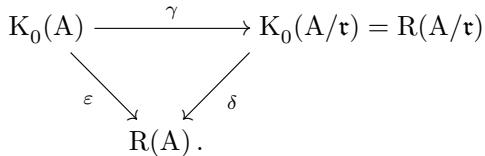
\includegraphics[keepaspectratio]{images/part002_05770a86.jpg}}

我们用 \(\mathcal{S}\) 表示单 A-模的类所成之（有限）集；对每个 \(\lambda \in \mathcal{S}\)，选取一个模 \(S_{\lambda}\)（其类为 \(\lambda\)）和一个投射覆盖 \((P_{\lambda}, u_{\lambda})\)（它覆盖 \(S_{\lambda}\)）（VIII, 第 175 页，命题 4）。由 VIII, 第 176 页的命题 6 得出，\(K_0(A)\) 是一个自由 \(\mathbf{Z}\)-模，以族 \(([P_{\lambda}]_{\mathcal{P}(A)})_{\lambda \in \mathcal{S}}\) 为基。此外，由于 \(S_{\lambda}\) 同构于 \(P_{\lambda} / \mathfrak{r}P_{\lambda}\)（VIII, 第 176 页），\(\gamma\) 把基 \(([P_{\lambda}]_{\mathcal{P}(A)})_{\lambda \in \mathcal{S}}\)（\(K_0(A)\) 的基）变为基 \(([S_{\lambda}])_{\lambda \in \mathcal{S}}\)（\(R(A / \mathfrak{r})\) 的基）。同构 \(\delta\) 把基 \(([S_{\lambda}])_{\lambda \in \mathcal{S}}\)（\(R(A / \mathfrak{r})\) 的基）变为基 \(([S_{\lambda}])_{\lambda \in \mathcal{S}}\)（\(R(A)\) 的基）。

A 的嘉当矩阵是矩阵 \((a_{\lambda\mu})\)，即 Z-模同态 \(\varepsilon: K_{0}(A) \to R(A)\) 关于基 \(([P_{\lambda}]_{\mathcal{P}(A)})_{\lambda \in \mathcal{S}}\)（\(K_{0}(A)\) 的基）与基 \(([S_{\lambda}])_{\lambda \in \mathcal{S}}\)（\(R(A)\) 的基）的矩阵。按定义，我们有

\[
[ \mathrm{P} _ {\mu} ] = \sum_ {\lambda \in \mathcal {S}} a _ {\lambda \mu} [ \mathrm{S} _ {\lambda} ] \quad (\mu \in \mathcal {S})\tag{19}
\]

（在群 R(A) 中）。换句话说，\(a_{\lambda\mu}\) 是同构于 \(S_{\lambda}\) 的商在 A-模 \(P_{\mu}\) 的某条若尔当–赫尔德列中的个数。

令 \(\pi = \varepsilon \circ \gamma^{-1} \circ \delta^{-1}\)；它是群 R(A) 的一个自同态。若 M 是一个有限生成半单 A-模且 (P, \(u\)) 是 M 的一个投射覆盖，则我们有 \(\pi([M]) = [P]\)。由公式 (19)，\(\pi\) 关于 R(A) 的基 \(([S_{\lambda}])_{\lambda \in \mathcal{S}}\) 的矩阵正是 A 的嘉当矩阵。

\subsection{\texorpdfstring{\(K_{0}(A)\) 的换环}{K\_\{0\}(A) 的换环}}

设 A 与 B 是环。设 \(f: A \to B\) 是一个环同态。若 P 是一个有限生成投射 A-模，则 B-模 \(f^{*}(P) = B \otimes_{A} P\) 是投射且有限生成的（II, §5, No.~2, 第 281 页，推论）。映射 \(P \mapsto \text{cl}(f^{*}(P))\) 是从幺半群 \(\mathcal{P}(A)\) 到幺半群 \(\mathcal{P}(B)\) 的一个同态，因此定义了一个同态 \(f^{*}: K_{0}(A) \to K_{0}(B)\)，它由关系式 \(f^{*}([P]_{\mathcal{P}(A)}) = [f^{*}(P)]_{\mathcal{P}(B)}\)（对每个有限生成投射 A-模 P）刻画。若 \(g: B \to C\) 是第二个环同态，则由标量扩张的递移性（II, §5, No.~1, 第 278 页，命题 2）得出，同态 \((g \circ f)^*\) 与 \(g^{*} \circ f^{*}\)（都是从 \(\mathrm{K}_{0}(\mathrm{A})\) 到 \(\mathrm{K}_{0}(\mathrm{C})\) 的同态）相等。

假设 \(f\) 使 B 成为一个有限生成投射左 A-模。设 Q 是一个有限生成投射左 B-模。则 Q 是一个有限生成自由 B-模的直因子，而后者作为 A-模是投射且有限生成的。于是，由 Q 经标量限制得到的 A-模 \(f_{*}(\mathrm{Q})\) 是投射且有限生成的。同上，我们导出一个同态 \(f_{*}: \mathrm{K}_{0}(\mathrm{B}) \to \mathrm{K}_{0}(\mathrm{A})\)，它由关系式 \(f_{*}([Q]_{\mathcal{P}(B)}) = [f_{*}(Q)]_{\mathcal{P}(A)}\)（对每个有限生成投射 B-模 Q）刻画。若 \(g: \mathrm{B} \to \mathrm{C}\) 是使 C 成为有限生成投射 B-模的环同态，则同态 \((g \circ f)_{*}\) 与 \(f_{*} \circ g_{*}\)（都是从 \(\mathrm{K}_{0}(\mathrm{C})\) 到 \(\mathrm{K}_{0}(\mathrm{A})\) 的同态）相等。

\subsection{弗罗贝尼乌斯互反律}

设 A 是一个半单环。设 f 是从 A 到半单环 B 的一个同态。设 S 是一个单 A-模，T 是一个单 B-模，且设 D 与 E 分别是 S 与 T 的中心化子。由舒尔引理（VIII, 第 47 页，推论），D 与 E 都是体。用 H 表示从 S 到 \(f_{*}(\mathrm{T})\) 的 A-线性同态所成之集。我们赋予 H 一个 (E,D)-双模结构，其外部合成律为 \((e,u)\mapsto e\circ u\) 与 \((d,u)\mapsto u\circ d\)（对 \(e\in E\)，\(u\in H\)，\(d\in D\)）。

命题 11. —— a) 重数 \([f_{*}(\mathrm{T}):\mathrm{S}]\)（单 A-模 S 在半单 A-模 \(f_{*}(\mathrm{T})\) 中的重数）等于把 H 视为 D 上右向量空间时的维数。

\begin{enumerate}
\def\labelenumi{\alph{enumi})}
\setcounter{enumi}{1}
\tightlist
\item
  重数 \([f^{*}(\mathrm{S}):\mathrm{T}]\) 是有限的，且等于把 H 视为 E 上左向量空间时的维数。
\end{enumerate}

断言 a) 由 VIII, 第 72 页的公式 (11) 得出。

B-模 \(f^{*}(S)\) 是半单且有限生成的，故具有有限长度。由同前所引的公式 (12)，我们有

\[
[ f ^ {*} (\mathrm{S}): \mathrm{T} ] = \dim_ {\mathrm{E}} \operatorname{Hom} _ {\mathrm{B}} (f ^ {*} (\mathrm{S}), \mathrm{T}).\tag{20}
\]

另外，在 II, §5, No.~1, 第 277--278 页的公式 (2) 与注 2 中，我们定义了一个从 \(\mathrm{Hom}_{\mathrm{A}}(\mathrm{S},f_{*}(\mathrm{T}))\) 到 \(\mathrm{Hom}_{\mathrm{B}}(f^{*}(\mathrm{S}),\mathrm{T})\) 的 E-线性双射。于是断言 b) 由公式 (20) 得出。

推论（弗罗贝尼乌斯互反律）. —— 假设 A 与 B 是交换域 K 上为有限维的半单代数，且 f 是 K-线性的。则 K-向量空间 S、T、D、E 与 H 都是有限维的，并且我们有等式

\[
[ f _ {*} (\mathrm{T}): \mathrm{S} ] [ \mathrm{D}: \mathrm{K} ] = [ f ^ {*} (\mathrm{S}): \mathrm{T} ] [ \mathrm{E}: \mathrm{K} ] = [ \mathrm{H}: \mathrm{K} ].\tag{21}
\]

特别地，当 K 是代数闭的时，我们有 D = E = K，且

\[
[ f _ {*} (\mathrm{T}): \mathrm{S} ] = [ f ^ {*} (\mathrm{S}): \mathrm{T} ] = [ \mathrm{H}: \mathrm{K} ].\tag{22}
\]

由于 A-模 S 是单的，它是单生成的，且 D 是 \(\operatorname{Hom}_{\mathrm{K}}(\mathrm{S},\mathrm{S})\) 的一个线性子空间；故 S 与 D 在 K 上都是有限维的。出于同样的理由，T 与 E 在 K 上是有限维的。最后，H 是 \(\operatorname{Hom}_{\mathrm{K}}(\mathrm{S},\mathrm{T})\) 的一个线性子空间；因而它也是有限维的。于是公式 (21) 由命题 11 得出，因为 H 在 K 上的维数等于 \([H:D][D:K]\)，也等于 \([H:E][E:K]\)（II, §1, No.~13, 第 222 页，命题 25）。由 VIII, 第 47 页的定理 1，若 K 是代数闭的，我们有 D = E = K。于是推论的第二部分由第一部分得出。

设 \(\mathrm{A}\) 与 \(\mathrm{B}\) 是交换域 \(\mathrm{K}\) 上为有限维的半单代数，且设 \(f\) 是一个 \(\mathrm{K}\)-代数同态（从 \(\mathrm{A}\) 到 \(\mathrm{B}\)）。

用 \(\mathcal{S}(\mathrm{A})\) 表示单 A-模的类所成之集；对每个 \(\lambda \in \mathcal{S}(\mathrm{A})\)，设 \(\mathrm{S}_{\lambda}\) 是类为 \(\lambda\) 的一个模，\(\mathrm{D}_{\lambda}\) 是它的中心化子。则 \(\mathrm{D}_{\lambda}\) 是 \(\mathrm{K}\) 上的一个有限次数代数；我们把这个次数记作 \(d_{\lambda}\)。我们类似地定义 \(\mathcal{S}(\mathrm{B})\)、\(\mathrm{T}_{\mu}\)、\(\mathrm{E}_{\mu}\) 与 \(e_{\mu}\)（对 \(\mu\) 属于 \(\mathcal{S}(\mathrm{B})\)）。格罗滕迪克群 \(\mathrm{K}_0(\mathrm{A})\) 以族 \(([\mathrm{S}_{\lambda}])_{\lambda \in \mathcal{S}(\mathrm{A})}\) 为基，而 \(\mathrm{K}_0(\mathrm{B})\) 以族 \(([\mathrm{T}_{\mu}])_{\mu \in \mathcal{S}(\mathrm{B})}\) 为基。设 \((a_{\mu \lambda})\) 是 \(f^{*}: \mathrm{K}_{0}(\mathrm{A}) \to \mathrm{K}_{0}(\mathrm{B})\) 关于这些基的矩阵，\((b_{\lambda \mu})\) 是 \(f_{*}: \mathrm{K}_{0}(\mathrm{B}) \to \mathrm{K}_{0}(\mathrm{A})\) 关于这些基的矩阵。按定义，我们有

\[
a _ {\mu \lambda} = [ f ^ {*} (\mathrm{S} _ {\lambda}): \mathrm{T} _ {\mu} ], \qquad b _ {\lambda \mu} = [ f _ {*} (\mathrm{T} _ {\mu}): \mathrm{S} _ {\lambda} ]\tag{23}
\]

（\(\lambda\) 属于 \(\mathcal{S}(\mathrm{A})\)，\(\mu\) 属于 \(\mathcal{S}(\mathrm{B})\)）。我们把向量空间 \(\mathrm{Hom}_{\mathrm{A}}(\mathrm{S}_{\lambda}, f_{*}(\mathrm{T}_{\mu}))\) 在域 K 上的维数记作 \(h_{\lambda \mu}\)。由上面的推论，我们有

\[
h _ {\lambda \mu} = e _ {\mu} a _ {\mu \lambda} = d _ {\lambda} b _ {\lambda \mu}.\tag{24}
\]

当域 K 是代数闭的时，我们有 \(d_{\lambda} = e_{\mu} = 1\)；于是，我们有

\[
a _ {\mu \lambda} = b _ {\lambda \mu} = h _ {\lambda \mu}.\tag{25}
\]

换句话说，\(f_{*}\) 与 \(f^{*}\) 关于 \(\mathrm{K}_0(\mathrm{A})\) 与 \(\mathrm{K}_0(\mathrm{B})\) 的给定基的矩阵互为转置。

\subsection{单环的情形}

设 A 与 B 是单环，f 是从 A 到 B 的一个同态。设 S 是一个单 A-模，T 是一个单 B-模。我们令

\[
i (f) = [ f ^ {*} (\mathrm{S}): \mathrm{T} ] = \mathrm{long} _ {\mathrm{B}} (f ^ {*} (\mathrm{S}));\tag{26}
\]

我们把基数 \(i(f)\) 称为 f 的指数。当 A 是 B 的子环且 f 是 A 到 B 中的典范单射时，我们把 \(i(\mathrm{B},\mathrm{A})\) 记作 \(i(f)\) 的替代，并把这个基数称为 A 在 B 中的指数。我们类似地定义 f 的高度 \(h(f)\)：

\[
h (f) = [ f _ {*} (\mathrm{T}): \mathrm{S} ] = \mathrm{long} _ {\mathrm{A}} (f _ {*} (\mathrm{T})).\tag{27}
\]

当 A 是 B 的子环且 f 是 A 到 B 中的典范单射时，我们用 \(h(\mathrm{B}, \mathrm{A})\) 表示 \(h(f)\)，并把它称为 A 在 B 中的高度。

A-模 S 是单生成的，故 B-模 \(f^{*}(\mathrm{S}) = \mathrm{B} \otimes_{\mathrm{A}} \mathrm{S}\) 亦然。由此得出 \(i(f)\) 是有限的，从而是一个整数。设 M 是一个 A-模。用 a 表示它的长度；则 M 同构于 \(\mathrm{S}^{(\mathfrak{a})}\)。于是 B-模 \(f_{*}(\mathrm{M})\) 同构于 \(f_{*}(\mathrm{S})^{(\mathfrak{a})}\)。由 \(i(f)\) 的定义，我们因此有

\[
\mathrm{long} _ {\mathrm{B}} (f ^ {*} (\mathrm{M})) = i (f) \mathrm{long} _ {\mathrm{A}} (\mathrm{M}).\tag{28}
\]

Z-模 \(K_{0}(A)\) 与 \(K_{0}(B)\) 都是维数为 1 的自由模，分别以 {[}S{]} 与 {[}T{]} 为基，并且我们有

\[
f ^ {*} ([ \mathrm{S} ]) = i (f) [ \mathrm{T} ].\tag{29}
\]

特别地，取 \(M = A_{s}\)；则 \(f^{*}(A_{s}) = B \otimes_{A} A_{s}\) 同构于 \(B_{s}\)（II, §3, No.~4, 第 249 页），故

\[
i (f) = \mathrm{long(B)} / \mathrm{long(A)}.\tag{30}
\]

由韦德伯恩定理（VIII, 第 120 页，定理 1），存在整数 \(m \geqslant 1\) 与 \(n \geqslant 1\) 以及体 D 与 E，使得 A 同构于 \(\mathbf{M}_m(\mathrm{D})\)，B 同构于 \(\mathbf{M}_n(\mathrm{E})\)。由公式 (30)，我们有 \(i(f) = n / m\)；特别地，\(m\) 整除 \(n\)。

设 N 是一个 B-模；用 a 表示它的长度。则 N 同构于 \(\mathrm{T}^{(\mathfrak{a})}\)，故 A-模 \(f_{*}(\mathrm{N})\) 同构于 \(f_{*}(\mathrm{T})^{(\mathfrak{a})}\)；由 \(h(f)\) 的定义，我们有

\[
\mathrm{long} _ {\mathrm{A}} (f _ {*} (\mathrm{N})) = h (f) \mathrm{long} _ {\mathrm{B}} (\mathrm{N}).\tag{31}
\]

我们已经看到（VIII, 第 124 页，命题 5），f 使 B 成为一个自由 A-模，且该模的所有基都具有同一基数，记作 \([B:A]_{s}\)，称为 B 在 A 上的（左）次数。A-模 \(f_{*}(B_{s})\) 同构于 \(A_{s}^{[B:A]_{s}}\)，故其长度为 \([B:A]_{s}\) long(A)。把公式 (30) 与公式 (31) 应用于特例 \(N=B_{s}\)，我们因此有

\[
[ \mathrm{B}: \mathrm{A} ] _ {s} = i (f) h (f).\tag{32}
\]

现在假设 B 是一个有限生成 A-模，即 \([B:A]_{s}\) 是有限的。则由公式 (32)，\(h(f)\) 是有限的。我们（在 VIII, 第 202 页）定义了一个群同态 \(f_{*}\)（从 \(K_{0}(B)\) 到 \(K_{0}(A)\)）；我们有

\[
f _ {*} ([ \mathrm{T} ]) = h (f) [ \mathrm{S} ].\tag{33}
\]

假设 A 与 B 是交换域 K 上为有限维的代数，且 f 是 K-线性的。同前，存在整数 \(m \geqslant 1\) 与 \(n \geqslant 1\)、为体的 K-代数 D 与 E，以及从 A 到 \(\mathbf{M}_{m}(\mathrm{D})\)、从 B 到 \(\mathbf{M}_{n}(\mathrm{E})\) 的 K-代数同构。令 \(d = [D : K]\) 且 \(e = [E : K]\)。我们于是有关系式

\[
[ \mathrm{A}: \mathrm{K} ] = m ^ {2} d, \qquad [ \mathrm{B}: \mathrm{K} ] = n ^ {2} e, \qquad [ \mathrm{B}: \mathrm{A} ] _ {s} = \frac {n ^ {2} e}{m ^ {2} d}
\]

以及，由公式 (30) 与 (32)，关系式

\[
i (f) = \frac {n}{m}, \qquad h (f) = \frac {n e}{m d}.
\]

当域 \(\mathrm{K}\) 是代数闭的时，我们有 \(d = e = 1\)，因此 \(i(f) = h(f)\) 且 \([\mathrm{B}:\mathrm{A}]_s = i(f)^2\)。

设 A、B 与 C 是单环，且设 \(f: A \to B\) 与 \(g: B \to C\) 是同态。设 S 是一个单 A-模。C-模 \((g \circ f)^{*}(S)\) 与 \(g^{*}(f^{*}(S))\) 同构；因此，由公式 (26) 与 (28)，我们有

\[
i (g \circ f) = \operatorname{long} _ {\mathrm{C}} \left(g ^ {*} \left(f ^ {*} (\mathrm{S})\right)\right) = i (g) \operatorname{long} _ {\mathrm{B}} \left(f ^ {*} (\mathrm{S})\right) = i (g) i (f).
\]

我们可以类似地证明等式 \(h(g \circ f) = h(g)h(f)\)。当 A 是 B 的子环且 B 是 C 的子环，并且对 f 与 g 取典范单射时，这些等式给出

\[
i (\mathrm{C}, \mathrm{A}) = i (\mathrm{C}, \mathrm{B}) i (\mathrm{B}, \mathrm{A}), \qquad h (\mathrm{C}, \mathrm{A}) = h (\mathrm{C}, \mathrm{B}) h (\mathrm{B}, \mathrm{A}).\tag{34}
\]

命题 12. —— 设 B 是一个单环，A 是 B 的一个单子环。假设 B 是一个有限生成左 A-模。设 M 是一个非零的有限生成左 B-模。令 \(A' = \text{End}_{A}(M)\) 且 \(B' = \text{End}_{B}(M)\)。则 \(B'\) 是 \(A'\) 的一个子环，环 \(A'\) 与 \(B'\) 都是单的，\(A'\) 是一个有限生成左 \(B'\)-模，并且我们有等式

\[
i (\mathrm{A} ^ {\prime}, \mathrm{B} ^ {\prime}) = h (\mathrm{B}, \mathrm{A}), \quad h (\mathrm{A} ^ {\prime}, \mathrm{B} ^ {\prime}) = i (\mathrm{B}, \mathrm{A}), \quad [ \mathrm{A} ^ {\prime}: \mathrm{B} ^ {\prime} ] _ {s} = [ \mathrm{B}: \mathrm{A} ] _ {s}.
\]

由 VIII, 第 123 页的命题 4，环 \(\mathrm{A}'\) 是单的，\(\mathrm{M}\) 是一个有限长度的 \(\mathrm{A}'\)-模，并且我们有

\[
\mathrm{long} _ {\mathrm{A}} (\mathrm{M}) = \mathrm{long} (\mathrm{A} ^ {\prime}), \quad \mathrm{long} _ {\mathrm{A} ^ {\prime}} (\mathrm{M}) = \mathrm{long} (\mathrm{A}).
\]

出于同样的理由，环 \(B'\) 是单的，并且我们有

\[
\operatorname{long} _ {\mathrm{B}} (\mathrm{M}) = \operatorname{long} \left(\mathrm{B} ^ {\prime}\right), \quad \operatorname{long} _ {\mathrm{B} ^ {\prime}} (\mathrm{M}) = \operatorname{long} (\mathrm{B}).
\]

于是，由公式 (31) 与 (30)，我们有

\[
h (\mathrm{B}, \mathrm{A}) = \operatorname{long} _ {\mathrm{A}} (\mathrm{M}) / \operatorname{long} _ {\mathrm{B}} (\mathrm{M}) = \operatorname{long} \left(\mathrm{A} ^ {\prime}\right) / \operatorname{long} \left(\mathrm{B} ^ {\prime}\right) = i \left(\mathrm{A} ^ {\prime}, \mathrm{B} ^ {\prime}\right);
\]

等式 \(h(\mathrm{A}^{\prime},\mathrm{B}^{\prime}) = i(\mathrm{B},\mathrm{A})\) 可以类似地建立。由此我们导出

\[
[ \mathrm{A} ^ {\prime}: \mathrm{B} ^ {\prime} ] _ {s} = i (\mathrm{A} ^ {\prime}, \mathrm{B} ^ {\prime}) h (\mathrm{A} ^ {\prime}, \mathrm{B} ^ {\prime}) = h (\mathrm{B}, \mathrm{A}) i (\mathrm{B}, \mathrm{A}) = [ \mathrm{B}: \mathrm{A} ] _ {s}
\]

（利用公式 (32)）。特别地，\(A'\) 是一个有限生成左 \(B'\)-模。

\BourbakiExercises{习题}

\begin{enumerate}
\def\labelenumi{\arabic{enumi})}
\tightlist
\item
  设 p 是一个素数。用 C 表示形如 \((\mathbf{Z}/p^{2}\mathbf{Z})^{n} \oplus (\mathbf{Z}/p^{3}\mathbf{Z})^{m}\)（\(n, m \in N\)）的 Z-模的类所成之集。
\end{enumerate}

\begin{enumerate}
\def\labelenumi{\alph{enumi})}
\item
  证明 \(\mathcal{C}\) 是加性的但不是遗传的。最小的遗传集 \(\mathcal{H}\)（它包含 \(\mathcal{C}\)）是什么？
\item
  证明 C 型模的每个短正合列都分裂。描述群 \(\mathrm{K}(\mathcal{C})\)。
\item
  构造一个正合列
\end{enumerate}

\[
0 \to \mathrm{M} _ {0} \to \mathrm{M} _ {1} \to \mathrm{M} _ {2} \to \mathrm{M} _ {3} \to \mathrm{M} _ {4} \to 0
\]

（由 C 型模组成），使得 \(M_{0} \oplus M_{2} \oplus M_{4}\) 与 \(M_{1} \oplus M_{3}\) 在 \(\mathrm{K}(\mathcal{C})\) 中的类不相同。

\begin{enumerate}
\def\labelenumi{\alph{enumi})}
\setcounter{enumi}{3}
\tightlist
\item
  从 \(\mathrm{K}(\mathcal{C})\) 到 \(\mathrm{K}(\mathcal{H})\) 的自然同态是否是单射？
\end{enumerate}

\begin{enumerate}
\def\labelenumi{\arabic{enumi})}
\setcounter{enumi}{1}
\item
  设 \(\mathrm{A}\) 是一个环，\(a\) 与 \(b\) 是 \(\mathrm{A}\) 中满足 \(ab = 1\) 与 \(ba \neq 1\) 的两个元素。证明 A-模 \(\mathrm{A}(1 - ba)\) 是投射的，并且它与零 A-模稳定同构。更精确地说，证明 A-模 \(\mathrm{A}_s\) 与 \(\mathrm{A}(1 - ba) \oplus \mathrm{A}_s\) 同构。
\item
  设 A 与 B 是环。用 A 与 B 的格罗滕迪克群确定格罗滕迪克群 \(R(A \times B)\) 与 \(K_{0}(A \times B)\)（都是 \(A \times B\) 的）。
\item
  设 A 与 B 是森田等价的环。证明群 R(A) 与 R(B) 同构。对 \(K_{0}(A)\) 与 \(K_{0}(B)\) 同样处理。
\item
  设 A 是一个环。用 \(\mathcal{I}(A)\) 表示由偶 \((n,p)\)（其中 n 是整数，p 是 \(M_{n}(A)\) 中的一个幂等元）组成的集。在 \(\mathcal{I}(A)\) 上定义一个加法：令 \((m,p)+(n,q)=(m+n,\begin{pmatrix} p & 0 \\ 0 & q \end{pmatrix})\)。
\end{enumerate}

\begin{enumerate}
\def\labelenumi{\alph{enumi})}
\item
  设 \(\mathcal{P}(A^{\circ})\) 是有限生成投射右 A-模的类所成的幺半群。设 \(\varphi: \mathcal{I}(A) \to \mathcal{P}(A^{\circ})\) 是由 \(\varphi(n,p) = \operatorname{cl}(\operatorname{Im}p)\) 定义的映射。证明 \(\varphi\) 是一个满同态，且元素 \((m,p)\) 与 \((n,q)\)（都属于 \(\mathcal{I}(A)\)）在 \(\varphi\) 下有相同的像当且仅当存在 \(a \in M_{m,n}(A)\) 与 \(b \in M_{n,m}(A)\)，使得 ab = p 且 ba = q。
\item
  由此推出群 \(K_{0}(A)\) 与 \(K_{0}(A^{\circ})\) 同构。
\end{enumerate}

\begin{enumerate}
\def\labelenumi{\arabic{enumi})}
\setcounter{enumi}{5}
\tightlist
\item
  设 A 是一个环，G 是一个交换群，T: A → G 是一个迹型映射（VIII, 第 115 页，习题 3）。对每个有限生成投射右 A-模 P，用
\end{enumerate}

\[
\mathrm{T} _ {\mathrm{P}}: \operatorname{End} _ {\mathrm{A}} (\mathrm{P} \oplus \mathrm{A} _ {d}) \longrightarrow \mathrm{G}
\]

表示扩张 T 的唯一迹型映射（同前所引），并用 \(\pi_{P}\) 表示 \(\operatorname{End}_{\mathrm{A}}(\mathrm{P} \oplus \mathrm{A}_{d})\) 中以 P 为像、以 \(A_{d}\) 为核的投影子。构造一个群同态 \(\widetilde{\mathrm{T}} : \mathrm{K}_{0}(\mathrm{A}) \to \mathrm{G}\)，使得对每个有限生成投射右 A-模 P，有 \(\widetilde{\mathrm{T}}([\mathrm{P}]) = \mathrm{T}_{\mathrm{P}}(\pi_{\mathrm{P}})\)。

\begin{enumerate}
\def\labelenumi{\arabic{enumi})}
\setcounter{enumi}{6}
\tightlist
\item
  设 I 是一个右有向集，\((\mathrm{A}_{i}, f_{ji})\) 是环的一个直接系统，A 是它的极限。证明 \(\mathrm{K}_{0}(\mathrm{A})\) 是群的直接系统 \((\mathrm{K}_{0}(\mathrm{A}_{i}), f_{ji}^{*})\) 的极限。
\end{enumerate}

¶ 8) 设 A、B 与 C 是环，\(f: \mathrm{A} \to \mathrm{C}\) 与 \(g: \mathrm{B} \to \mathrm{C}\) 是环同态；假设 \(f\) 是满射。考虑 \(\mathrm{A} \times \mathrm{B}\) 中由偶 \((a, b)\)（满足 \(f(a) = g(b)\)）组成的子环 D。设 M 是一个 A-模，N 是一个 B-模，\(u\) 是从 \(\mathrm{C} \otimes_{\mathrm{A}} \mathrm{M}\) 到 \(\mathrm{C} \otimes_{\mathrm{B}} \mathrm{N}\) 的一个 C-同构。用 P 表示 \(\mathrm{M} \times \mathrm{N}\) 中由偶 \((m, n)\)（满足 \(u(1 \otimes m) = 1 \otimes n\)）组成的 D-子模。

\begin{enumerate}
\def\labelenumi{\alph{enumi})}
\item
  假设模 M 与 N 分别具有有限基 \((e_{i})_{i\in\mathrm{I}}\) 与 \((f_{j})_{j\in\mathrm{J}}\)，并且 u 在基 \((1\otimes e_{i})\) 与 \((1\otimes f_{j})\) 下的矩阵是一个以 A 为元素的逆矩阵 \((a_{ji})\) 的像。证明 D-模 P 是自由的；更精确地说，元素 \((e_{i},\sum_{j}a_{ji}f_{j})_{i\in\mathrm{I}}\) 构成 P 的一个基。
\item
  设 p 与 q 是整数，\(X \in \mathbf{M}_{p,q}(\mathrm{C})\) 与 \(Y \in \mathbf{M}_{q,p}(\mathrm{C})\) 是满足 \(XY = I_{p}\) 与 \(YX = I_{q}\) 的矩阵。证明方阵 \(\begin{pmatrix} X & 0 \\ 0 & Y \end{pmatrix}\) 是某个以 A 为元素的逆矩阵的像，利用恒等式
\end{enumerate}

\[
\left( \begin{array}{c c} X & 0 \\ 0 & Y \end{array} \right) = \left( \begin{array}{c c} I _ {p} & X \\ 0 & I _ {q} \end{array} \right) \left( \begin{array}{c c} I _ {p} & 0 \\ - Y & I _ {q} \end{array} \right) \left( \begin{array}{c c} I _ {p} & X \\ 0 & I _ {q} \end{array} \right) \left( \begin{array}{c c} 0 & - I _ {p} \\ I _ {q} & 0 \end{array} \right).
\]

\begin{enumerate}
\def\labelenumi{\alph{enumi})}
\setcounter{enumi}{2}
\item
  假设模 M 与 N 是自由且有限生成的。由 a) 与 b) 推出 D-模 P 是投射且有限生成的。
\item
  假设 M 与 N 是投射且有限生成的。构造一个 A-模 \(M'\) 与一个 B-模 \(N'\)，使得 \(M \oplus M'\) 与 \(N \oplus N'\) 是自由且有限生成的，并且 C-模 \(C \otimes_{A} M'\) 与 \(C \otimes_{B} N'\) 同构。由此推出 D-模 P 是投射且有限生成的。
\item
  证明由两个投射导出的典范同态 \(A \otimes_{D} P \to M\) 与 \(B \otimes_{D} P \to N\) 是双射（如上那样化归为 a) 的条件成立的情形）。
\item
  反之，设 \(P'\) 是一个有限生成投射 D-模；令 \(M' = A \otimes_{D} P'\) 与 \(N' = B \otimes_{D} P'\)，并用 \(u' : C \otimes_{A} M' \to C \otimes_{B} N'\) 表示典范同构。证明从 \(P'\) 到 \(M' \times N'\) 的典范同态诱导一个从 \(P'\) 到与 \((M', N', u')\) 相伴的 D-模上的 D-线性同构。
\end{enumerate}

\(g)\) 用 \(\varphi_0:\mathrm{K}_0(\mathrm{D})\to \mathrm{K}_0(\mathrm{A})\times \mathrm{K}_0(\mathrm{B})\) 与 \(\psi_0:\mathrm{K}_0(\mathrm{A})\times \mathrm{K}_0(\mathrm{B})\to \mathrm{K}_0(\mathrm{C})\) 表示满足

\[
\varphi_ {0} ([ \mathrm{P} ]) = ([ \mathrm{A} \otimes_ {\mathrm{D}} \mathrm{P} ], [ \mathrm{B} \otimes_ {\mathrm{D}} \mathrm{P} ]) \quad \text { and } \quad \psi_ {0} ([ \mathrm{M} ], [ \mathrm{N} ]) = [ \mathrm{C} \otimes_ {\mathrm{A}} \mathrm{M} ] - [ \mathrm{C} \otimes_ {\mathrm{B}} \mathrm{N} ].
\]

证明序列

\[
\mathrm{K} _ {0} (\mathrm{D}) \xrightarrow {\varphi_ {0}} \mathrm{K} _ {0} (\mathrm{A}) \times \mathrm{K} _ {0} (\mathrm{B}) \xrightarrow {\psi_ {0}} \mathrm{K} _ {0} (\mathrm{C})
\]

是正合的。证明若此外还存在一个环同态 \(s: C \to A\) 使得 \(f \circ s = Id_{C}\)，则 \(\varphi_{0}\) 是单射且 \(\psi_{0}\) 是满射。

\begin{enumerate}
\def\labelenumi{\arabic{enumi})}
\setcounter{enumi}{8}
\tightlist
\item
  设 A 是一个伪环，即一个结合的但不必含单位元的 Z-代数，\(\widetilde{A}\) 是由 A 通过添加单位元（III, §1, No.~2, 第 431 页）得到的 Z-代数；集合 \(\widetilde{\mathrm{A}}\) 等于 \(\mathbf{Z} \times \mathrm{A}\)。把同态 \((n, a) \mapsto n\) 记作 \(\varepsilon : \widetilde{\mathrm{A}} \to \mathbf{Z}\)，并把同态 \(\varepsilon^{*} : \mathrm{K}_{0}(\widetilde{\mathrm{A}}) \to \mathrm{K}_{0}(\mathbf{Z})\)（它与 \(\varepsilon\) 相伴）的核记作 \(\mathrm{K}_{0}(\mathrm{A})\)。
\end{enumerate}

\begin{enumerate}
\def\labelenumi{\alph{enumi})}
\item
  证明若 A 含单位元，则 \(\tilde{A}\) 同构于积环 \(Z \times A\)，且 \(K_{0}(A)\) 的这一定义与 No.~8 中给出的定义相容。
\item
  设 A 与 B 是伪环，\(f: \mathrm{A} \to \mathrm{B}\) 是一个同态。设 \(\widetilde{f}: \widetilde{\mathrm{A}} \to \widetilde{\mathrm{B}}\) 是由 \(\widetilde{f}((n, a)) = (n, f(a))\) 定义的环同态。证明 \(\widetilde{f}^*\) 把 \(\mathrm{K}_0(\mathrm{A})\) 映到 \(\mathrm{K}_0(\mathrm{B})\) 之中。把由 \(\widetilde{f}^*\) 导出的同态记作 \(f^*: \mathrm{K}_0(\mathrm{A}) \to \mathrm{K}_0(\mathrm{B})\)。c) 假设 \(f\) 是满射；用 \(\mathfrak{a}\) 表示它的核，并把 \(\mathfrak{a}\) 到 A 中的典范单射记作 \(i\)。证明序列
\end{enumerate}

\[
\mathrm{K} _ {0} (\mathfrak {a}) \xrightarrow {i ^ {*}} \mathrm{K} _ {0} (\mathrm{A}) \xrightarrow {f ^ {*}} \mathrm{K} _ {0} (\mathrm{B})
\]

是正合的。若此外还存在伪环的同态 \(s: B \to A\) 使得 \(f \circ s = Id_{B}\)，则 \(i^{*}\) 是单射且 \(f^{*}\) 是满射（对三元组 (A, B, C) 先取 (A, A, B) 再取 (D, Z, A)，应用习题 8）。

\begin{enumerate}
\def\labelenumi{\alph{enumi})}
\setcounter{enumi}{3}
\tightlist
\item
  证明习题 7 与 8 的结论可推广到伪环的情形。e) 用 \(\mathbf{M}_{\infty}(\mathrm{A})\) 表示以 A 为元素且仅有有限多个非零元素的 \(\mathbf{N} \times \mathbf{N}\) 矩阵所成的伪环。设 \(f: \mathrm{A} \to \mathbf{M}_{\infty}(\mathrm{A})\) 是把 \(a \in \mathrm{A}\) 映到矩阵 \((b_{ij})\)（满足 \(b_{00} = a\) 与 \(b_{ij} = 0\)，当 \((i,j) \neq (0,0)\)）的映射。证明 \(f^{*}\) 是从 \(\mathrm{K}_0(\mathrm{A})\) 到 \(\mathrm{K}_0(\mathbf{M}_{\infty}(\mathrm{A}))\) 的同构（利用习题 4 与 7）。
\end{enumerate}

\begin{enumerate}
\def\labelenumi{\arabic{enumi})}
\setcounter{enumi}{9}
\tightlist
\item
  设 A 是一个环。用 \(\mathbf{GL}_{\infty}(\mathrm{A})\) 表示 \(\mathbf{GL}(\mathrm{A}^{(\mathbf{N})})\) 中由满足 X - I 仅有有限多个非零元素的矩阵 X 组成的子群，并用 \(\mathrm{E}(\mathrm{A})\) 表示 \(\mathbf{GL}_{\infty}(\mathrm{A})\) 中由形如 \(I + \lambda E_{ij}\)（其中 i, j 属于 N，\(i \neq j\)，\(\lambda \in A\)）的矩阵生成的子群；它是 \(\mathbf{GL}_{\infty}(\mathrm{A})\) 的导群（II, §10, 第 422 页，习题 15）。把商群 \(\mathbf{GL}_{\infty}(\mathrm{A}) / \mathrm{E}(\mathrm{A})\) 记作 \(\mathrm{K}_{1}(\mathrm{A})\)；它的群运算写作加法。每个环同态 \(f : A \to B\) 诱导一个群同态 \(f^{*} : K_{1}(A) \to K_{1}(B)\)。
\end{enumerate}

\begin{enumerate}
\def\labelenumi{\alph{enumi})}
\item
  对每个整数 \(n \geqslant 1\)，设 \(\iota_{n} : \mathbf{GL}_{n}(\mathrm{A}) \to \mathrm{K}_{1}(\mathrm{A})\) 是把 \(X \in \mathbf{GL}_{n}(\mathrm{A})\) 映到矩阵 \(\begin{pmatrix} X & 0 \\ 0 & I \end{pmatrix}\) 的类的同态。证明若环 A 是局部环，则对每个 n，\(\iota_{n}\) 是满射（利用 VIII, 第 42 页，习题 17）。
\item
  假设环 A 是交换的。构造一个满同态 \(d_{\mathrm{A}} : \mathrm{K}_{1}(\mathrm{A}) \to \mathrm{A}^{*}\)，使得对每个 n 有 \(d_{A} \circ \iota_{n} = det\)。若此外 A 是局部环或欧几里得环，则同态 \(d_{A}\) 与 \(\iota_{1}\) 是互逆的双射。
\item
  设 I 是一个右有向集，\((\mathrm{A}_{i}, f_{ji})\) 是环的一个直接系统，A 是它的极限。证明 \(\mathrm{K}_{1}(\mathrm{A})\) 是群的直接系统 \((\mathrm{K}_{1}(\mathrm{A}_{i}), f_{ji}^{*})\) 的极限。
\end{enumerate}

¶ 11) 采用习题 8 的假设与记号。用 \(f': \mathrm{D} \to \mathrm{B}\) 与 \(g': \mathrm{D} \to \mathrm{A}\) 表示由两个投射导出的同态，并用

\[
\varphi_ {1}: \mathrm{K} _ {1} (\mathrm{D}) \rightarrow \mathrm{K} _ {1} (\mathrm{A}) \times \mathrm{K} _ {1} (\mathrm{B}) \quad \text { and } \quad \psi_ {1}: \mathrm{K} _ {1} (\mathrm{A}) \times \mathrm{K} _ {1} (\mathrm{B}) \rightarrow \mathrm{K} _ {1} (\mathrm{C})
\]

表示由 \(\varphi_1(z) = (g'^* (z), f'^* (z))\) 与 \(\psi_1(x,y) = f^* (x) - g^* (y)\) 定义的映射。

\begin{enumerate}
\def\labelenumi{\alph{enumi})}
\tightlist
\item
  证明序列
\end{enumerate}

\[
\mathrm{K} _ {1} (\mathrm{D}) \xrightarrow {\varphi_ {1}} \mathrm{K} _ {1} (\mathrm{A}) \times \mathrm{K} _ {1} (\mathrm{B}) \xrightarrow {\psi_ {1}} \mathrm{K} _ {1} (\mathrm{C})
\]

是正合的（注意 \(f(\mathrm{E}(\mathrm{A})) = \mathrm{E}(\mathrm{C})\)）。证明若此外还存在一个环同态 \(s : C \to A\) 使得 \(f \circ s = Id_{C}\)，则 \(\psi_{1}\) 是满射。

\begin{enumerate}
\def\labelenumi{\alph{enumi})}
\setcounter{enumi}{1}
\item
  对每个整数 n 与 \(\mathbf{GL}_{n}(\mathrm{C})\) 的每个元素 g，用 \(P_{g}\) 表示与模 \(A^{n}\)、\(B^{n}\) 以及从 \(C \otimes_{A} A^{n}\) 到 \(C \otimes_{B} B^{n}\) 的以 g 为矩阵的同构相伴的投射 D-模（习题 8）。构造一个同态 \(\partial : K_{1}(\mathrm{C}) \to K_{0}(\mathrm{D})\)，使得 \(\partial \circ \iota_{n}(g) = [\mathrm{P}_{g}] - [\mathrm{D}_{s}^{n}]\) 对每个整数 n 与 \(\mathbf{GL}_{n}(\mathrm{C})\) 的每个元素 g 成立。
\item
  证明序列
\end{enumerate}

\[
\mathrm{K} _ {1} (\mathrm{D}) \xrightarrow {\varphi_ {1}} \mathrm{K} _ {1} (\mathrm{A}) \times \mathrm{K} _ {1} (\mathrm{B}) \xrightarrow {\psi_ {1}} \mathrm{K} _ {1} (\mathrm{C}) \xrightarrow {\partial} \mathrm{K} _ {0} (\mathrm{D}) \xrightarrow {\varphi_ {0}} \mathrm{K} _ {0} (\mathrm{A}) \times \mathrm{K} _ {0} (\mathrm{B}) \xrightarrow {\psi_ {0}} \mathrm{K} _ {0} (\mathrm{C})
\]

是正合的。

\begin{enumerate}
\def\labelenumi{\arabic{enumi})}
\setcounter{enumi}{11}
\tightlist
\item
  设 \(f: \mathrm{A} \to \mathrm{B}\) 是一个满射环同态，\(\mathfrak{a}\) 是其核，且 \(i\) 是从 \(\mathfrak{a}\) 到 \(\mathrm{A}\) 的典范单射。构造一个同态 \(\partial: \mathrm{K}_1(\mathrm{B}) \to \mathrm{K}_0(\mathfrak{a})\)，使得序列
\end{enumerate}

\[
\mathrm{K} _ {1} (\mathrm{A}) \xrightarrow {f ^ {*}} \mathrm{K} _ {1} (\mathrm{B}) \xrightarrow {\partial} \mathrm{K} _ {0} (\mathfrak {a}) \xrightarrow {i ^ {*}} \mathrm{K} _ {0} (\mathrm{A}) \xrightarrow {f ^ {*}} \mathrm{K} _ {0} (\mathrm{B})
\]

是正合的（按习题 11, c) 的方式论证）。

\begin{enumerate}
\def\labelenumi{\arabic{enumi})}
\setcounter{enumi}{12}
\item
  用 \(\mathcal{C}\)（相应地，\(\mathcal{D}\)）表示有限长度 \(\mathbf{Z}\)-模（相应地，有限生成 \(\mathbf{Z}\)-模）的类所成之集。证明群同态 \(\gamma_{\mathcal{D},\mathcal{C}}\)（从 \(\mathrm{K}(\mathcal{C})\) 到 \(\mathrm{K}(\mathcal{D})\)）是零同态。
\item
  设 K 是一个特征异于 2 的交换域。令
\end{enumerate}

\[
\mathrm{A} = \mathrm{K} [ \mathrm{X}, \mathrm{Y}, \mathrm{Z} ] / (\mathrm{X} ^ {2} + \mathrm{Y} ^ {2} + \mathrm{Z} ^ {2} - 1).
\]

设 M 是 A-模 \(\mathrm{A}^{3}/\mathrm{A}(\overline{\mathrm{X}},\overline{\mathrm{Y}},\overline{\mathrm{Z}})\)，其中 \(\overline{X}\)、\(\overline{Y}\) 与 \(\overline{Z}\) 分别表示 X、Y 与 Z 在 A 中的像。证明 \(M\oplus A\) 是自由 A-模，但 M 不是自由模。

\section{半单模的张量积}

在本节中，字母 K 表示一个交换域。若 E 与 F 是 K 上的向量空间，则我们把张量积 \(E \otimes_{K} F\) 记作 \(E \otimes F\)。

\subsection{代数的张量积上的半单模}

在本小节中，我们考虑 K-代数 \(A_{1}\) 与 \(A_{2}\)；我们把代数 \(A_{1} \otimes A_{2}\) 记作 A。

命题 1. —— 设 \(M_{1}\) 是一个 \(A_{1}\)-模，\(M_{2}\) 是一个 \(A_{2}\)-模，二者都不约化为 0。若模 \(M = M_{1} \otimes M_{2}\)（环 \(A = A_{1} \otimes A_{2}\) 上的模）是单模（相应地，同构模、半单模），则 \(A_{1}\)-模 \(M_{1}\) 与 \(A_{2}\)-模 \(M_{2}\) 是单模（相应地，同构模、半单模）。

假设 M 是半单 A-模。设 \(N_{1}\) 是一个 \(A_{1}\)-子模（\(M_{1}\) 的）。用 N 表示 \(N_{1} \otimes M_{2}\) 在 A-模 M 中的典范像。由 VIII, 第 56 页，推论 2，存在 M 中一个以 N 为像的 A-线性投影子 p。由假设，\(M_{2} \neq 0\)；因此可以选取 \(M_{2}\) 的一个元素 m 和一个线性形式 \(\varphi\)（在 K-向量空间 \(M_{2}\) 上，满足 \(\varphi(m) = 1\)）（II, §7, No.~5, 第 302 页，推论 2）。设 u 是从 \(M_{1}\) 到 M 的映射，由 \(u(m_{1}) = m_{1} \otimes m\) 定义；v 是从 M 到 \(M_{1}\) 的 K-线性映射，由 \(v(m_{1} \otimes m_{2}) = \varphi(m_{2})m_{1}\) 刻画。令 \(q = v \circ p \circ u\)。映射 \(q : M_{1} \to M_{1}\) 是 \(A_{1}\)-线性的，它的像含于 \(N_{1}\)，并且我们有 \(q(n) = n\)（对每个 \(n \in N_{1}\)）。于是，q 是 \(M_{1}\) 中以 \(N_{1}\) 为像的投影子。我们证明了 \(M_{1}\) 是半单 \(A_{1}\)-模（VIII, 第 56 页，推论 2）。

假设 M 是单模，且 \(M_{1}\) 是两个 \(A_{1}\)-子模 \(M_{1}^{\prime}\) 与 \(M_{1}^{\prime\prime}\) 的直和。令 \(M^{\prime}=M_{1}^{\prime}\otimes M_{2}\) 与 \(M^{\prime\prime}=M_{1}^{\prime\prime}\otimes M_{2}\)；则 M 是 A-子模 \(M'\) 与 \(M''\) 的直和。由于 M 是单模，\(M'\) 或 \(M''\) 必约化为 0；由假设 \(M_{2} \neq 0\)，故 \(M_{1}' = 0\) 或 \(M_{1}'' = 0\)（II, §3, No.~7, 第 256 页，推论 2）。这就证明了 \(M_{1}\) 是单 \(A_{1}\)-模。

现在假设 M 是同构 A-模。设 S 与 T 是两个单 \(A_{1}\)-子模（属于 \(M_{1}\)）。于是 A-模 \(S \otimes M_{2}\) 与 \(T \otimes M_{2}\) 可与 M 的非零子模视为同一。因而它们是与 M 同型的同构模。由注 VIII, 第 61 页，存在一个非零 A-线性映射 \(f : S \otimes M_{2} \to T \otimes M_{2}\)。映射 f 特别还是 \(A_{1}\)-线性的。由于 \(A_{1}\)-模 \(S \otimes M_{2}\) 与 \(T \otimes M_{2}\) 非零，且分别是 S 型与 T 型的同构模，故 S 与 T 同构。这就证明了 \(M_{1}\) 是同构 \(A_{1}\)-模。

命题 2. —— 设 S 是环 \(A = A_{1} \otimes A_{2}\) 上的一个单模，在 K 上有限维。对 \(i \in \{1, 2\}\)，存在一个单 \(A_{i}\)-模 \(S_{i}\)，使得 \(A_{i}\)-模 S 是 \(S_{i}\) 型的同构模。A-模 S 同构于 A-模 \(S_{1} \otimes S_{2}\) 的一个商。

由于 S 是一个在 K 上有限维的非零 \(A_{1}\)-模，它在 \(A_{1}\) 上有有限长度，且存在一个单左 \(A_{1}\)-模 \(S_{1}\) 以及一个非零 \(A_{1}\)-线性映射（从 \(S_{1}\) 到 S）。我们赋予 \(\mathrm{M}_{2} = \mathrm{Hom}_{\mathrm{A}_{1}}(\mathrm{S}_{1}, \mathrm{S})\) 一个左 \(A_{2}\)-模结构，它由外合成律 \((a_{2}, u) \mapsto (a_{2})_{\mathrm{S}} \circ u\) 定义。由构造，\(M_{2} \neq 0\)，且 \(M_{2}\) 在 K 上有限维。因此可以找到一个单左 \(A_{2}\)-模 \(S_{2}\) 与一个非零 \(A_{2}\)-线性映射 \(\varphi : S_{2} \to M_{2}\)。我们定义一个非零 A-线性映射 \(\psi\)（从 \(S_{1} \otimes S_{2}\) 到 S），由

\[
\psi (s _ {1} \otimes s _ {2}) = \varphi (s _ {2}) (s _ {1})\tag{1}
\]

（对每个 \(s_{1} \in S_{1}\) 与 \(s_{2} \in S_{2}\)）。由于 S 是单 A-模且 \(\psi\) 非零，\(\psi\) 是满射，从而 S 同构于 \(S_{1} \otimes S_{2}\) 的一个商。对 \(i \in \{1, 2\}\)，\(A_{i}\)-模 \(S_{1} \otimes S_{2}\) 是 \(S_{i}\) 型的同构模，因此 \(A_{i}\)-模 S 亦然（VIII, 第 61 页，命题 2）。

对任意 K-代数 B，我们用 \(\mathcal{S}_{\mathrm{K}}(\mathrm{B})\) 表示在 K 上有限维的单（VIII, 第 51 页）左 B-模的类所成之集。

定理 1. —— 假设体 K 是代数封闭的。

\begin{enumerate}
\def\labelenumi{\alph{enumi})}
\item
  设 \(M_{1}\) 是一个 \(A_{1}\)-模，\(M_{2}\) 是一个 \(A_{2}\)-模，二者都是在 K 上有限维的单模（相应地，半单模）。则 \(M_{1} \otimes M_{2}\) 是环 \(A_{1} \otimes A_{2}\) 上的单模（相应地，半单模），且在 K 上有限维。
\item
  从 \(\mathcal{S}_{\mathrm{K}}(\mathrm{A}_1)\times \mathcal{S}_{\mathrm{K}}(\mathrm{A}_2)\) 到 \(\mathcal{S}_{\mathrm{K}}(\mathrm{A}_1\otimes \mathrm{A}_2)\) 的、把 \((\operatorname {cl}(\mathrm{S}_1),\operatorname {cl}(\mathrm{S}_2))\) 映到 \(\operatorname {cl}(\mathrm{S}_1\otimes \mathrm{S}_2)\) 的映射（其中 \(\mathrm{S}_1\)（相应地，\(\mathrm{S}_2\)）是单 \(\mathrm{A}_1\)-模（相应地，单 \(\mathrm{A}_2\)-模），且在 \(\mathrm{K}\) 上有限维）是双射。
\end{enumerate}

为证明 a)，只需考虑 \(M_{1}\) 与 \(M_{2}\) 都是单模的情形。设 \(M'\) 是 \(M = M_{1} \otimes M_{2}\) 的一个 A-子模；它是一个 \(A_{1}\)-子模（属于 \(M_{1} \otimes M_{2}\)），在形如 \(1_{M_{1}} \otimes u\)（其中 u 取遍 \(A_{2}\)-模 \(M_{2}\) 的位似所成之集）的自同态集下稳定。由于体 K 是代数封闭的，舒尔引理（VIII, 第 47 页，定理 1）蕴含交换子 \(\operatorname{End}_{\mathrm{A}_{1}}(\mathrm{M}_{1})\)（即 \(M_{1}\) 的交换子）等于 K。由 VIII, 第 63 页，推论 2，A-子模 \(M'\)（\(M_{1} \otimes M_{2}\) 的）形如 \(M_{1} \otimes M_{2}'\)，其中 \(M_{2}'\) 是一个 \(A_{2}\)-子模（\(M_{2}\) 的）。我们已假设 \(M_{2}\) 是单模；因此 \(M_{2}' = 0\) 或 \(M_{2}' = M_{2}\)，即 \(M' = 0\) 或 \(M' = M\)。于是，M 是单模。

若 S 是 \(A_{1} \otimes A_{2}\) 上在 K 上有限维的单模，则由命题 2 与 a) 可知，S 同构于形如 \(S_{1} \otimes S_{2}\) 的模，其中 \(S_{1}\)（相应地，\(S_{2}\)）是单 \(A_{1}\)-模（相应地，单 \(A_{2}\)-模）。此外，作为 \(A_{i}\)-模，S 是 \(S_{i}\) 型的同构模，故 \(S_{i}\) 的类只依赖于 S 的类。这就证明了 b)。

注. —— 1) 当不假设体 K 代数封闭时，定理 1 的断言 a) 不再成立。可以举出这样的例子（VIII, 第 225 页，习题 4）：\(M_{i}\) 是在 K 上有限维的单 \(A_{i}\)-模（对 \(i \in \{1, 2\}\)），而 A-模 \(M_{1} \otimes M_{2}\) 不是半单的，或者是半单的但不是单的。

\begin{enumerate}
\def\labelenumi{\arabic{enumi})}
\setcounter{enumi}{1}
\tightlist
\item
  存在一个同态 \(\varphi\)（从 \(\mathrm{R_K(A_1)\otimes_{\mathbf{Z}} R_K(A_2)}\) 到 \(\mathrm{R_K(A)}\)），由关系式 \(\varphi ([\mathrm{M}_1]\otimes [\mathrm{M}_2]) = [\mathrm{M}_1\otimes \mathrm{M}_2]\) 刻画。这可以用与 VIII, 第 196 页，命题 9 相同的方式证明。若体 \(K\) 是代数封闭的，则由定理 1, b)，\(\varphi\) 是从 \(\mathrm{R_K(A_1)\otimes_{\mathbf{Z}} R_K(A_2)}\) 到 \(\mathrm{R_K(A)}\) 的同构，因为对每个 K-代数 B，\(\mathbf{Z}\)-模 \(\mathrm{R_K(B)}\) 是自由的，以族 \(([\mathrm{S}])_{\mathrm{S}\in \mathcal{S}_{\mathrm{K}}(\mathrm{B})}\) 为基（VIII, 第 195 页）。
\end{enumerate}

\subsection{单模的张量积}

设 \(A_{1}\) 与 \(A_{2}\) 是交换域 K 上的代数。我们把 K-代数 \(A_{1} \otimes A_{2}\) 记作 A。

引理 1. —— 设 \(M_{1}\) 与 \(N_{1}\) 是 \(A_{1}\)-模，\(M_{2}\) 与 \(N_{2}\) 是 \(A_{2}\)-模。我们作如下假设：

\begin{enumerate}
\def\labelenumi{(\roman{enumi})}
\item
  \(A_{1}\)-模 \(M_{1}\) 是有限生成的。
\item
  \(A_{2}\)-模 \(M_{2}\) 是有限生成的，或者 \(N_{1}\) 在 K 上有限维。
\end{enumerate}

令 \(\mathrm{M} = \mathrm{M}_1\otimes \mathrm{M}_2\) 与 \(\mathrm{N} = \mathrm{N}_1\otimes \mathrm{N}_2\)，并把它们视为环 \(\mathrm{A} = \mathrm{A}_1\otimes \mathrm{A}_2\) 上的模。典范同态（II, §3, No.~5, 第 251 页）

\[
\lambda : \operatorname{Hom} _ {\mathrm{K}} (\mathrm{M} _ {1}, \mathrm{N} _ {1}) \otimes \operatorname{Hom} _ {\mathrm{K}} (\mathrm{M} _ {2}, \mathrm{N} _ {2}) \longrightarrow \operatorname{Hom} _ {\mathrm{K}} (\mathrm{M}, \mathrm{N})
\]

于是诱导 K-向量空间的一个同构

\[
\varphi : \operatorname{Hom} _ {\mathrm{A} _ {1}} (\mathrm{M} _ {1}, \mathrm{N} _ {1}) \otimes \operatorname{Hom} _ {\mathrm{A} _ {2}} (\mathrm{M} _ {2}, \mathrm{N} _ {2}) \longrightarrow \operatorname{Hom} _ {\mathrm{A}} (\mathrm{M}, \mathrm{N}).
\]

映射 \(\lambda\) 是单射（II, §7, No.~7, 第 308 页，命题 16），并把线性子空间 \(\mathrm{Hom}_{\mathrm{A}_1}(\mathrm{M}_1,\mathrm{N}_1)\otimes \mathrm{Hom}_{\mathrm{A}_2}(\mathrm{M}_2,\mathrm{N}_2)\) 映到 \(\mathrm{Hom}_{\mathrm{A}}(\mathrm{M},\mathrm{N})\)。因此只需证明每个从 M 到 N 的 A-线性映射都属于 \(\mathrm{Hom}_{\mathrm{A}_1}(\mathrm{M}_1,\mathrm{N}_1)\otimes \mathrm{Hom}_{\mathrm{A}_2}(\mathrm{M}_2,\mathrm{N}_2)\) 在 \(\lambda\) 下的像。设 \(u:\mathrm{M}\to \mathrm{N}\) 是一个 A-线性映射。设 \(x\in \mathrm{M}_1\)。用 \(u_{x}\) 表示 \(\mathrm{A}_2\)-线性映射 \(y\mapsto u(x\otimes y)\)（从 \(\mathrm{M}_2\) 到 \(\mathrm{N}_1\otimes \mathrm{N}_2\)）。令 \(\mathrm{P} = \mathrm{Hom}_{\mathrm{A}_2}(\mathrm{M}_2,\mathrm{N}_2)\)，并用 \(\nu\) 表示从 \(\mathrm{N}_1\otimes \mathrm{P}\) 到 \(\mathrm{Hom}_{\mathrm{A}_2}(\mathrm{M}_2,\mathrm{N}_1\otimes \mathrm{N}_2)\) 的典范同态（II, §4, No.~2, 第 269 页）。这个映射是单射（II, §4, No.~2, 第 269 页，命题 2, (i)，应用于 K-向量空间 \(\mathbf{N}_1\)）。由假设 (ii)，存在一个线性子空间 \(\mathrm{V}_x\)（\(\mathbf{N}_1\) 的，在 K 上有限维），使得 \(u_{x}\) 取值于 \(\mathrm{V}_x\otimes \mathrm{N}_2\)。由此可知，\(u_{x}\) 是 \(\nu\) 下某个唯一元素 \(v_{x}\)（属于 \(\mathbf{N}_1\otimes \mathbf{P}\)）的像。映射 \(\widetilde{u}:x\mapsto v_x\)（从 \(\mathbf{M}_1\) 到 \(\mathbf{N}_1\otimes \mathbf{P}\)）是 \(\mathbf{A}_1\)-线性的。由假设 (i)，\(\mathbf{A}_1\)-模 \(\mathbf{M}_1\) 是有限生成的。与上面类似的论证表明，\(\widetilde{u}\) 属于 \(\mathrm{Hom}_{\mathrm{A}_1}(\mathrm{M}_1,\mathrm{N}_1)\otimes \mathrm{P}\) 在 \(\mathrm{Hom}_{\mathrm{A}_1}(\mathrm{M}_1,\mathrm{N}_1\otimes \mathrm{P})\) 中的像。引理 1 得证。

定理 2. —— 设 \(A_{1}\) 与 \(A_{2}\) 是交换域 K 上的代数；设 \(S_{1}\) 是单 \(A_{1}\)-模，\(S_{2}\) 是单 \(A_{2}\)-模。设 \(D_{1}\) 与 \(D_{2}\) 分别是 \(S_{1}\) 与 \(S_{2}\) 的交换子。令 \(M = S_{1} \otimes S_{2}\)，\(A = A_{1} \otimes A_{2}\)，\(D = D_{1} \otimes D_{2}\)。我们把 M 视为左 (A,D)-双模。

\begin{enumerate}
\def\labelenumi{\alph{enumi})}
\item
  A-模 M 的交换子等于 \(\mathrm{D}_{\mathrm{M}}\)。
\item
  映射 \(a \mapsto aM\) 是从按包含关系排序的 D 的右理想所成之集到按包含关系排序的 M 的 A-子模所成之集的同构。逆映射把 M 的子模 N 映到由满足 \(dM \subset N\) 的元素 d 组成的 D 的理想。
\end{enumerate}

断言 a) 由引理 1 得出，因为单模是单生成的。

设 \(\mathrm{T}\) 是 \((\mathrm{A}_1, \mathrm{D}_2)\)-双模 \(\mathrm{S}_1 \otimes (\mathrm{D}_2)_d\)。我们把 \(\mathrm{M} = \mathrm{S}_1 \otimes \mathrm{S}_2\) 与 \(\mathrm{T} \otimes_{\mathrm{D}_2} \mathrm{S}_2\) 视为同一（II, §3, No.~8, 第 258 页）；这一视为同一与环 \(\mathrm{A} = \mathrm{A}_1 \otimes \mathrm{A}_2\) 上的左模结构相容。

设 \(\mathrm{N}\) 是 \(\mathrm{M}\) 的一个 A-子模；它是 \(\mathrm{A}_2\)-子模（属于 \(\mathrm{T} \otimes_{\mathrm{D}_2} \mathrm{S}_2\)），在形如 \((a_1)_\mathrm{T} \otimes 1_{\mathrm{S}_2}\)（其中 \(a_1\) 取遍 \(\mathrm{A}_1\)）的自同态下稳定。由 VIII, 第 63 页，推论 2，存在唯一的 \((\mathrm{A}_1, \mathrm{D}_2)\)-子双模 \(\mathrm{V}\)（\(\mathrm{T}\) 的），使得 \(\mathrm{N} = \mathrm{V} \otimes_{\mathrm{D}_2} \mathrm{S}_2\)。

同构 \(u\)（从 \(\mathrm{T} = \mathrm{S}_1 \otimes (\mathrm{D}_2)_d\) 到 \(((\mathrm{D}_1)_d \otimes (\mathrm{D}_2)_d) \otimes_{\mathrm{D}_1} \mathrm{S}_1\)，由 \(u(s \otimes d) = 1 \otimes d \otimes s\) 定义）是 \((\mathrm{A}_1, \mathrm{D}_2)\)-线性的。我们把这些 \((\mathrm{A}_1, \mathrm{D}_2)\)-双模视为同一。与上面给出的论证类似，可以证明存在唯一的右 \((\mathrm{D}_1 \otimes \mathrm{D}_2)\)-子模 \(\mathfrak{a}\)（\(\mathrm{D}_1 \otimes \mathrm{D}_2\) 的），使得 \(\mathrm{V} = \mathfrak{a} \otimes_{\mathrm{D}_1} \mathrm{S}_1\)。考虑到上面所作的视为同一，\(\mathfrak{a}\) 是 \(\mathrm{D} = \mathrm{D}_1 \otimes \mathrm{D}_2\) 的唯一使得 \(\mathrm{N} = \mathfrak{a}\mathrm{M}\) 的右理想。

我们刚刚证明了映射 \(a \mapsto aM\) 是双射；最后的断言由此得出。

推论 1. —— 模 \(S_{1} \otimes S_{2}\)（环 \(A_{1} \otimes A_{2}\) 上的）是半单的（相应地，同型的、单的）当且仅当环 \(D = D_{1} \otimes D_{2}\) 是半单的（相应地，单环、体）。特别地，\(S_{1} \otimes S_{2}\) 是单模（当 \(S_{1}\) 或 \(S_{2}\) 的交换子等于 K 时）。

由定理 2，模 \(S_{1} \otimes S_{2}\)（环 \(D_{1} \otimes D_{2}\) 上的）是半单的（相应地，同型的、单的）当且仅当右 D-模 \((\mathrm{D}_{1} \otimes \mathrm{D}_{2})_{d}\) 是（VIII, 第 109 页，命题 10）。而右 D-模 \(D_{d}\) 是单模当且仅当 D 是体；它是同型的（相应地，半单的）当且仅当环 D 是单环（相应地，半单环）（VIII, 第 120 页，定义 1；VIII, 第 121 页，推论 1；以及 VIII, 第 137 页，命题 2）。

推论 2. —— 我们有 \(\mathfrak{R}_{\mathrm{A}}(\mathrm{M}) = \mathfrak{R}(\mathrm{D})\mathrm{M}\)。A-模 M 无根当且仅当环 D 无根。

这由 VIII, 第 108 页，命题 8 与定理 2, b) 得出。

\subsection{半单交换代数的张量积}

定理 3. —— 设 \(\mathbf{Z}_1\) 与 \(\mathbf{Z}_2\) 是 \(\mathbf{K}\) 上的半单交换代数。环 \(\mathbf{Z}_1 \otimes \mathbf{Z}_2\) 的根等于它的幂零元素所成之集。

我们先处理 \(Z_{1}\) 与 \(Z_{2}\) 是体 K 的扩张 \(L_{1}\) 与 \(L_{2}\) 的情形。必要时交换 \(L_{1}\) 与 \(L_{2}\)，可化归为 \(L_{1}\) 在 K 上的超越次数小于 \(L_{2}\) 在 K 上的超越次数的情形。

选取一个代数闭包 \(\Omega\)（\(\mathrm{L}_2\) 的）；由 V, §14, No.~6, 第 114 页，定理 5 的推论 1，我们可以假设 \(\mathrm{L}_1\) 是 \(\Omega\) 的一个子扩张。

\begin{enumerate}
\def\labelenumi{\Alph{enumi})}
\item
  我们先证明 \(L_{1} \otimes L_{2}\) 的根含于 \(L_{1} \otimes \Omega\) 的根。令 \(\mathfrak{a} = \Re(L_{1} \otimes L_{2})(L_{1} \otimes \Omega)\)；它是交换环 \(L_{1} \otimes \Omega\) 的一个理想，我们必须证明 a 含于 \(L_{1} \otimes \Omega\) 的根。换句话说（VIII, 第 156 页，定理 1），我们必须证明对 \(x \in a\)，元素 \(1 + x\) 在 \(L_{1} \otimes \Omega\) 中可逆。由于 \(\Omega\) 是 \(L_{2}\) 的代数扩张，存在一个有限次数的扩张 \(L_{3}\)（\(L_{2}\) 的），使得 x 属于 \(\Re(L_{1} \otimes L_{2})(L_{1} \otimes L_{3})\)。显然只需证明 \(1 + x\) 在 \(L_{1} \otimes L_{3}\) 中可逆。而 \(C = L_{1} \otimes L_{3}\) 是环 \(B = L_{1} \otimes L_{2}\) 上的一个有限生成模。由 VIII, 第 175 页的推论，我们有 \(\Re(B)C \subset \Re(C)\)，故 x 属于 C 的根，从而 \(1 + x\) 在 C 中可逆。
\item
  我们来证明 \(L_{1} \otimes \Omega\) 的根由幂零元素组成。用 p 表示 K 的特征指数，用 P 表示 K 在 \(\Omega\) 中的相对 p-根式（即纯不可分）闭包（V, §5, No.~2, 第 25 页）；体 P 是完备的。由于 P 是 K 的代数扩张，我们有 \(\mathrm{L}_{1}(\mathrm{P}) = \mathrm{L}_{1}[\mathrm{P}]\)（V, §3, No.~2, 第 18 页，推论 1）。设 b 是从 \(L_{1} \otimes P\) 到体 \(P_{1} = L_{1}[P]\) 的典范同态的核。设 \(x \in b\)；存在元素 \(y_{1}, \ldots, y_{n}\)（\(L_{1}\) 的）与元素 \(z_{1}, \ldots, z_{n}\)（P 的），使得 \(x = \sum_{i=1}^{n} y_{i} \otimes z_{i}\) 且 \(\sum_{i=1}^{n} y_{i} z_{i} = 0\)。由于 P 在 K 上是 p-根式的，存在 p 的一个幂 q，使得 \(z_{1}^{q}, \ldots, z_{n}^{q}\) 属于 K。于是我们有
\end{enumerate}

\[
x ^ {q} = \sum_ {i = 1} ^ {n} y _ {i} ^ {q} \otimes z _ {i} ^ {q} = \sum_ {i = 1} ^ {n} y _ {i} ^ {q} z _ {i} ^ {q} \otimes 1 = \left(\sum_ {i = 1} ^ {n} y _ {i} z _ {i}\right) ^ {q} \otimes 1 = 0.
\]

所以 b 由幂零元素组成。

令 \(c = b \otimes_{P} \Omega\)；它是从 \((\mathrm{L}_{1} \otimes \mathrm{P}) \otimes_{\mathrm{P}} \Omega\) 到 \(P_{1} \otimes_{P} \Omega\) 的典范同态的核，且由上面的论证知它由幂零元素组成。而 \(\Omega\) 是 P 的代数封闭扩张，\(P_{1}\) 是 \(\Omega\) 的一个子扩张。由于体 P 是完备的，\(P_{1}\) 是 P 的可分扩张（V, §15, No.~5, 第 125 页，定理 3）。由 V, 第 120 页，定理 4，交换环 \(P_{1} \otimes_{P} \Omega\) 的诸极大理想之交约化为 0。换句话说，环 \(P_{1} \otimes_{P} \Omega\)（它同构于 \(((L_{1} \otimes P) \otimes_{P} \Omega)/c\)）是无根的。这就证明（VIII, 第 155 页，命题 5）c 包含环 \((\mathrm{L}_{1} \otimes \mathrm{P}) \otimes_{\mathrm{P}} \Omega\) 的根。而这一环同构于 \(L_{1} \otimes \Omega\)，且 c 由幂零元素组成。因此，\(L_{1} \otimes \Omega\) 的根由幂零元素组成。

\begin{enumerate}
\def\labelenumi{\Alph{enumi})}
\setcounter{enumi}{2}
\tightlist
\item
  特殊情形证明的结尾。由 A) 与 B)，根 \(\mathfrak{r}\)（\(\mathrm{L}_1\otimes \mathrm{L}_2\) 的）含于这一交换环的幂零元素所成之集 \(\mathfrak{n}\)。此外我们知道 \(\mathfrak{n}\) 含于 \(\mathfrak{r}\)（VIII, 第 157 页，注 2）。
\end{enumerate}

现在考虑一般情形。由于半单交换 K-代数是体 K 的有限多个扩张的积（VIII, 第 137 页，命题 3），且环的积的根是诸根的积（VIII, 第 156 页，推论 3），\(Z_{1} \otimes Z_{2}\) 的根是这一环的幂零元素所成之集。

\subsection{代数的张量积的根}

设 \(A_{1}\) 与 \(A_{2}\) 是 K-代数，令 \(A = A_{1} \otimes A_{2}\)。

命题 3. —— 假设代数 \(\mathrm{A}_1\) 与 \(\mathrm{A}_2\) 是半单的，其中心分别为 \(\mathbf{Z}_1\) 与 \(\mathbf{Z}_2\)。令 \(\mathbf{Z} = \mathbf{Z}_1 \otimes \mathbf{Z}_2\)。

\begin{enumerate}
\def\labelenumi{\alph{enumi})}
\item
  映射 \(a \mapsto aA\) 是从按包含关系排序的 Z 的理想所成之集到按包含关系排序的 A 的双边理想所成之集的同构。
\item
  A 的根等于 A 的诸极大双边理想之交，且等于 \(\Re(Z)A\)。
\item
  若 K-代数 \(Z_{1}\) 与 \(Z_{2}\) 之一是可分的，特别地若体 K 是完备的，则环 Z 与 A 的根均约化为 0。
\end{enumerate}

每个代数 \(A_{i}\) 都是有限多个单代数的积。而环的积的中心是诸中心的积，且对根（VIII, 第 156 页，推论 3）与对双边理想（I, §8, No.~10, 第 109 页，命题 8）也有类似的断言。因此只需在 \(A_{1}\) 与 \(A_{2}\) 都是单代数的假设下证明命题 3。

对 \(i \in \{1,2\}\)，令 \(B_i = A_i \otimes A_i^o\)，并把 \(A_i\) 视为一个 \(B_i\)-模，其中位似由公式

\[
(x \otimes y) z = x z y
\]

给出，其中 x、y 与 z 属于 \(A_{i}\)。\(B_{i}\)-模 \(A_{i}\) 的交换子是 \((\mathrm{Z}_{i})_{\mathrm{A}_{i}}\)，即由 \(Z_{i}\) 的元素作的位似所成之集；我们把它与 \(Z_{i}\) 视为同一。此外，\(B_{i}\)-子模（\(A_{i}\) 的）就是 \(A_{i}\) 的双边理想，且由于环 \(A_{i}\) 是单环，仅有的双边理想是 0 与 \(A_{i}\)。因而 \(A_{i}\) 是单 \(B_{i}\)-模。再者，\((\mathrm{B}_{1}\otimes\mathrm{B}_{2})\)-子模（\(A_{1}\otimes A_{2}\) 的）就是环 \(A_{1}\otimes A_{2}\) 的双边理想。

于是，把 VIII, 第 214 页，定理 2, b) 应用于单 \(\mathrm{B}_1\)-模 \(\mathrm{A}_1\)（交换子为 \(\mathrm{Z}_1\)）以及单 \(\mathrm{B}_2\)-模 \(\mathrm{A}_2\)（交换子为 \(\mathrm{Z}_2\)），即得断言 a)。

我们来证明断言 b)。A 的诸极大双边理想之交是 \((\mathrm{B}_{1}\otimes\mathrm{B}_{2})\)-模 \(A_{1}\otimes A_{2}\) 的根；由 VIII, 第 215 页，推论 2，这一交与 \(\Re(\mathrm{Z})\mathrm{A}\) 重合。代数 \(Z_{1}\) 与 \(Z_{2}\) 是交换且半单的。因此环 Z 的根由幂零元素组成（VIII, 第 215 页，定理 3），且环 A 的双边理想 \(\Re(\mathrm{Z})\mathrm{A}\) 含于根 \(\Re(\mathrm{A})\)（VIII, 第 157 页，注 1）。然而，A 的诸极大双边理想之交包含 \(\Re(\mathrm{A})\)（VIII, 第 155 页，命题 5, d)）。这就证明了断言 b)。

可分交换代数与既约交换代数的张量积是既约环（V, §15, No.~2, 第 120 页，命题 5）。代数 \(Z_1\) 与 \(Z_2\) 是交换且半单的，因而是既约的。若代数 \(Z_1\) 与 \(Z_2\) 之一是可分的，则代数 \(Z\) 是既约的；于是由 VIII, 第 215 页，定理 3，它是无根的，且我们有 \(\Re(A) = \Re(Z)A = 0\)。特别地，当体 \(K\) 完备时即属此种情形，因为完备体上的每个既约交换代数都是可分的（V, §15, No.~5, 第 125 页，定理 3）。

推论. —— 假设代数 \(A_{1}\) 与 \(A_{2}\) 都是单的，且中心 \(Z_{1}\)（\(A_{1}\) 的）约化为 K。则环 \(A_{1} \otimes A_{2}\) 除 0 与其自身外没有其他双边理想。

由假设，\(Z_{1} = K\)，且由于 \(A_{2}\) 是单的，其中心 \(Z_{2}\) 是一个体（VIII, 第 121 页，推论 1, a)）。因此环 \(Z = Z_{1} \otimes Z_{2}\) 是体，推论由命题 3, a) 得出。

\subsection{半单模的张量积}

命题 4. —— 对 \(i \in \{1,2\}\)，设 \(\mathrm{A}_i\) 是一个 K-代数，\(\mathrm{M}_i\) 是一个半单 \(\mathrm{A}_i\)-模，\(\mathrm{Z}_i\) 是 \(\mathrm{M}_i\) 的交换子的中心。令 \(\mathrm{A} = \mathrm{A}_1 \otimes \mathrm{A}_2\)，\(\mathrm{M} = \mathrm{M}_1 \otimes \mathrm{M}_2\)，\(\mathrm{Z} = \mathrm{Z}_1 \otimes \mathrm{Z}_2\)。我们有 \(\Re_{\mathrm{A}}(\mathrm{M}) = \Re(\mathrm{Z})\mathrm{M}\)。若代数 \(\mathrm{Z}_1\) 与 \(\mathrm{Z}_2\) 之一在 \(\mathrm{K}\) 上可分，特别地若体 \(\mathrm{K}\) 是完备的，则 A-模 \(\mathrm{M}\) 无根。

对 \(i \in \{1,2\}\)，设 \(S_i\) 是一个单 \(A_i\)-模，\(D_i\) 是它的交换子，\(I(i)\) 是一个集合。我们先处理 \(M_i\) 是 \(A_i\)-模 \(S_i^{(I(i))}\) 的情形。我们把它的交换子的中心 \(Z_i\) 与 \(D_i\) 的中心视为同一。令 \(D = D_1 \otimes D_2\)。

我们有 \(\Re (\mathrm{D}) = \Re (\mathrm{Z})\mathrm{D}\)（VIII, 第 217 页，命题 3）与 \(\Re_{\mathrm{A}}(\mathrm{S}_1\otimes \mathrm{S}_2) =\) \(\Re (\mathrm{D})(\mathrm{S}_1\otimes \mathrm{S}_2)\)（VIII, 第 215 页，推论 2），因而 \(\Re_{\mathrm{A}}(\mathrm{S}_1\otimes \mathrm{S}_2) = \Re (\mathrm{Z})(\mathrm{S}_1\otimes \mathrm{S}_2)\)。A-模 M 是一族同构于 \(\mathrm{S}_1\otimes \mathrm{S}_2\) 的 A-模的直和，而一族模的直和的根是诸根的直和（VIII, 第 152 页，推论 2）。因此我们有 \(\Re_{\mathrm{A}}(\mathrm{M}) = \Re (\mathrm{Z})\mathrm{M}\)。

现在考虑一般情形。对 \(i \in \{1,2\}\)，把 \(A_{i}\)-模 \(M_{i}\) 的支集记作 \(S_{M_{i}}\)。对 \(\lambda \in S_{M_{i}}\)，把 \(M_{i}\) 的 \(\lambda\) 型同型分量记作 \(M_{i;\lambda}\)，并把它的交换子的中心记作 \(Z_{i;\lambda}\)。我们把环 \(Z_{i}\) 与诸环 \(Z_{i;\lambda}\)（\(\lambda \in S_{M_{i}}\)）的积视为同一。设 \(\lambda \in S_{M_{1}}\) 与 \(\mu \in S_{M_{2}}\)。用 \(i_{\lambda}: Z_{1;\lambda} \to Z_{1}\) 表示唯一的 K-线性映射，使得 \(pr_{\lambda} \circ i_{\lambda}\) 是 \(Z_{1;\lambda}\) 上的恒同映射，且 \(pr_{\lambda'} \circ i_{\lambda}\) 是零映射（对 \(\lambda' \in S_{M_{1}} = \{\lambda\}\)）。同样地定义 \(i_{\mu}: Z_{2;\mu} \to Z_{2}\)。令 \(Z_{\lambda,\mu} = Z_{1;\lambda} \otimes Z_{2;\mu}\) 与 \(i_{\lambda,\mu} = i_{\lambda} \otimes i_{\mu}\)，并把映射 \(pr_{\lambda} \otimes pr_{\mu}\)（从 Z 到 \(Z_{\lambda,\mu}\)）记作 \(\pi_{\lambda,\mu}\)。映射 \(\pi_{\lambda,\mu}\) 是一个满射环同态；因此我们有 \(\pi_{\lambda,\mu}(\Re(Z)) \subset \Re(Z_{\lambda,\mu})\)（VIII, 第 155 页，命题 5, b)）。我们来证明反包含。设 z 是 \(\Re(Z_{\lambda,\mu})\) 的一个元素；由于 \(Z_{1;\lambda}\) 与 \(Z_{2;\mu}\) 都是体，z 是幂零的（VIII, 第 215 页，定理 3）。我们有 \(i_{\lambda,\mu}(xy) = i_{\lambda,\mu}(x) \cdot i_{\lambda,\mu}(y)\)（对 \(Z_{\lambda,\mu}\) 中的 x、y）；因此 \(i_{\lambda,\mu}(z)\) 是幂零的，从而属于 \(\Re(Z)\)。由于 \(\pi_{\lambda,\mu} \circ i_{\lambda,\mu}\) 是 \(Z_{\lambda,\mu}\) 上的恒同映射，元素 z 属于 \(\pi_{\lambda,\mu}(\Re(Z))\)。我们就这样证明了等式 \(\pi_{\lambda,\mu}(\Re(Z)) = \Re(Z_{\lambda,\mu})\)。

令 \(M_{\lambda,\mu}=M_{1;\lambda}\otimes M_{2;\mu}\)；这是 M 的一个在 Z 下稳定的子模。对 \(z\in Z\) 与 \(m\in M_{\lambda,\mu}\)，我们有 \(zm=\pi_{\lambda,\mu}(z)m\)。因此，\(\Re(Z)M_{\lambda,\mu}\) 等于 \(\Re(Z_{\lambda,\mu})M_{\lambda,\mu}\)，从而由同型情形知等于 \(\Re_{A}(M_{\lambda,\mu})\)。由于直和的根是诸根的直和（VIII, 第 152 页，推论 2），且 M 是诸子模 \(M_{\lambda,\mu}\)（\((\lambda,\mu)\in\mathcal{S}_{\mathrm{M}_{1}}\times\mathcal{S}_{\mathrm{M}_{2}}\)）的直和，等式 \(\Re_{A}(M)=\Re(Z)M\) 得证。最后的断言则由 VIII, 第 217 页，命题 3 得出。

引理 2. —— 设 \(A_{1}\) 与 \(A_{2}\) 是交换域 K 上的代数。设 \(M_{1}\) 是一个在 K 上有限维的 \(A_{1}\)-模，\(M_{2}\) 是一个有限长度的 \(A_{2}\)-模。则 \(A_{1} \otimes A_{2}\)-模 \(M_{1} \otimes M_{2}\) 具有有限长度。

令 \(M = M_{1} \otimes M_{2}\)。设 \((e_{1}, \ldots, e_{n})\) 是 \(M_{1}\) 在体 K 上的一个基。映射 \((x_{1}, \ldots, x_{n}) \mapsto \sum_{i=1}^{n} e_{i} \otimes x_{i}\) 是从 \(A_{2}\)-模 \(M_{2}^{n}\) 到 \(A_{2}\)-模 M 的同构。由于 \(M_{2}\) 是有限长度的 \(A_{2}\)-模，M 亦然。此外，M 的每个 A-子模都是 \(A_{2}\)-子模；因此 M 是有限长度的 A-模。

命题 5. —— 设 \(A_{1}\) 与 \(A_{2}\) 是交换域 K 上的代数。设 \(M_{1}\) 是一个在 K 上有限维的半单 \(A_{1}\)-模，\(M_{2}\) 是一个半单 \(A_{2}\)-模。对 \(i \in \{1,2\}\)，把 \(A_{i}\)-模 \(M_{i}\) 的交换子记作 \(D_{i}\)，并把 \(D_{i}\) 的中心记作 \(Z_{i}\)。令 \(A = A_{1} \otimes A_{2}\)，\(M = M_{1} \otimes M_{2}\)，\(D = D_{1} \otimes D_{2}\)，\(Z = Z_{1} \otimes Z_{2}\)。

\begin{enumerate}
\def\labelenumi{\alph{enumi})}
\item
  A-模 M 的交换子可与 D 视为同一，它的中心是 Z。若 \(A_{2}\)-模 \(M_{2}\) 具有有限长度，则 A-模 M 具有有限长度，环 D 是右且左阿廷的，环 Z 是阿廷的。
\item
  下列性质等价：
\end{enumerate}

\begin{enumerate}
\def\labelenumi{(\roman{enumi})}
\item
  A-模 M 是半单的。
\item
  环 \(Z\) 同构于一族交换域的积。
\item
  环 Z 是既约的。
\end{enumerate}

\begin{enumerate}
\def\labelenumi{\alph{enumi})}
\setcounter{enumi}{2}
\tightlist
\item
  下列性质等价：
\end{enumerate}

\begin{enumerate}
\def\labelenumi{(\roman{enumi})}
\item
  A-模 M 是同型的且不约化为 0。
\item
  环 Z 是一个体。
\item
  环 \(\mathbf{Z}\) 是一个整环。
\end{enumerate}

由假设，\(M_{1}\) 在 K 上有限维。因此 M 的交换子可与 D 视为同一（VIII, 第 213 页，引理 1），且它的中心是 Z（III, §4, No.~4, 第 468 页，推论）。假设 \(A_{2}\)-模 \(M_{2}\) 具有有限长度。由引理 2，A-模 M 具有有限长度。由于 \(M_{2}\) 是半单且有限生成的，环 \(D_{2}\) 是半单的（VIII, 第 139 页，命题 6），且它的中心 \(Z_{2}\) 是有限族交换域的积。于是，\(D_{2}\)-模 \((\mathrm{D}_{2})_{s}\) 与 \(Z_{2}\)-模 \((\mathrm{Z}_{2})_{s}\) 都具有有限长度。此外，由于 \(M_{1}\) 在 K 上有限维，\(D_{1}\) 与 \(Z_{1}\) 亦然。由引理 2，模 \((\mathrm{D}_{1} \otimes \mathrm{D}_{2})_{s}\) 具有有限长度；因此环 \(D_{1} \otimes D_{2}\) 是左阿廷的。我们同样可证环 \(D_{1} \otimes D_{2}\) 是右阿廷的，且环 \(Z_{1} \otimes Z_{2}\) 是阿廷的。断言 a) 得证。

我们来证明 b)。半单模的交换子的中心同构于一族交换域的积（VIII, 第 87 页，命题 8, a)）；这就证明了 (i) 蕴含 (ii)。蕴含关系 (ii) \(\Rightarrow\) (iii) 是明显的。

假设环 Z 是既约的。则我们有 \(\Re(Z)=0\)（VIII, 第 215 页，定理 3）与 \(\Re_{\mathrm{A}}(\mathrm{M})=0\)（VIII, 第 218 页，命题 4）。由于 \(A_{2}\)-模 \(M_{2}\) 是半单的，存在一个族 \((\mathrm{S}_{i})_{i\in\mathrm{I}}\)（由单 \(A_{2}\)-模组成）以及一个从 \(M_{2}\) 到 \(\bigoplus S_{i}\) 的同构。因此，A-模 M 同构于 \(\bigoplus M_{1}\otimes S_{i}\)。于是对每个 \(i\in I\)，A-模 \(M_{1}\otimes S_{i}\) 无根。由 a)，它具有有限长度；故它是半单的（VIII, 第 153 页，命题 3, b)）。于是 A-模 M 是一族半单模的直和，从而是半单的。这就证明了 (iii) 蕴含 (i)，并完成了 b) 的证明。

一个 A-模是同型的且非零的，当且仅当它是半单的且其交换子的中心是一个体（VIII, 第 87 页，命题 8, b)）。于是 c) 由 b) 得出。

推论. —— 若 \(Z_{1}\) 或 \(Z_{2}\) 是体 K 上的可分代数（例如当 K 完备时即属此种情形），则 A-模 \(M_{1} \otimes M_{2}\) 是半单的。

环 \(Z_{1}\) 与 \(Z_{2}\) 同构于诸体的积，因而是既约环。特别地，若 K 是完备的，则它们是 K 上的可分代数（V, §15, No.~5, 第 125 页，定理 3）。由 V, §15, No.~2, 第 120 页，命题 5，可分代数与既约代数的张量积是既约的。于是 Z 是既约环，推论由命题 5, b) 得出。

\subsection{半单代数的张量积}

命题 6. —— 设 \(A_{1}\) 与 \(A_{2}\) 是非零 K-代数。若环 \(A_{1} \otimes A_{2}\) 是单的（相应地，半单的），则环 \(A_{1}\) 与 \(A_{2}\) 是单的（相应地，半单的）。

环 B 是半单的（相应地，单的）当且仅当 B-模 \(B_{s}\) 是半单的（相应地，同型的且非零）。因此本命题由（VIII, 第 211 页）命题 1 得出。

命题 7. —— 设 \(A_{1}\) 与 \(A_{2}\) 是半单 K-代数，其中心分别为 \(Z_{1}\) 与 \(Z_{2}\)。假设 \(A_{1}\) 在 K 上有有限次数。则环 \(A_{1} \otimes A_{2}\) 是左阿廷的，其中心 \(Z_{1} \otimes Z_{2}\) 亦然。环 \(A_{1} \otimes A_{2}\) 是单的（相应地，半单的）当且仅当环 \(Z_{1} \otimes Z_{2}\) 是一个体（相应地，既约环）。

这是 VIII, 第 219 页，命题 5 当 \(\mathrm{M}_1 = (\mathrm{A}_1)_s\)、\(\mathrm{M}_2 = (\mathrm{A}_2)_s\) 的情形。

推论 1. —— 设 \(A_{1}\) 与 \(A_{2}\) 是半单 K-代数；假设 \(A_{1}\) 在 K 上有限维。假设 \(A_{1}\) 或 \(A_{2}\) 的中心是 K 上的可分代数（例如当 K 完备时即属此种情形）。则 \(A_{1} \otimes A_{2}\) 是半单的。

这是 VIII, 第 221 页的推论当 \(\mathrm{M}_{1}=(\mathrm{A}_{1})_{s},\mathrm{M}_{2}=(\mathrm{A}_{2})_{s}\) 的情形。

推论 2. —— 设 \(A_{1}\) 与 \(A_{2}\) 是单 K-代数；假设 \(A_{1}\) 在 K 上有限维。若 \(A_{1}\) 或 \(A_{2}\) 的中心等于 K，则代数 \(A_{1} \otimes A_{2}\) 是单的。特别地，当 K 是代数封闭的时即属此种情形。

中心 \(Z_{1}\) 与 \(Z_{2}\)（相应地，\(A_{1}\) 与 \(A_{2}\) 的中心）都是体；若环 \(Z_{1}\) 与 \(Z_{2}\) 之一等于 K，则环 \(Z_{1} \otimes Z_{2}\) 是一个体。因此只需应用命题 7。

若体 \(\mathrm{K}\) 是代数封闭的，则 \(\mathrm{A}_1\) 的中心等于 \(\mathrm{K}\)。
